\documentclass[12pt]{article}
\usepackage{ctex}
\usepackage{amsmath}
\usepackage{siunitx}        
\usepackage{enumerate}
\usepackage{enumitem}
\usepackage{graphicx}
\usepackage{longtable}
\usepackage{booktabs}
\usepackage{CJK}
\usepackage{float}
\usepackage{titling}
\usepackage{fancyhdr}
\usepackage{setspace}
\usepackage{hyperref}
\usepackage{listings}
\usepackage{xcolor}
\usepackage{zhnumber} 
\usepackage{titlesec}
\usepackage[a4paper, left=2.5cm, right=2.5cm, top=3cm, bottom=3cm]{geometry}
\hypersetup{
	colorlinks=true,
	linkcolor=black,
	filecolor=magenta,      
	urlcolor=cyan,
}
\newcommand{\code}[1]{\texttt{#1}} % 用于排版代码/函数名

\renewcommand\thesection{\zhnum{section}}
\renewcommand\thesubsection{\arabic{section}.\arabic{subsection}}
\renewcommand\thesubsubsection{\arabic{section}.\arabic{subsection}.\arabic{subsubsection}}

\titleformat{\section}
{\centering\Large\bfseries}  % 格式:居中、大号、加粗
{\thesection}                % 保留章节编号
{0em}                        % 编号与标题之间的间距
{}


\hypersetup{
	pdfborder={0 0 0},  % 关闭边框
}

\title{ \textbf{基于分层优化与逆向建模的战场无人机投放策略}}
\date{}

\renewcommand{\abstractname}{\Large 摘要} 



\begin{document}
	\begin{CJK}{UTF8}{gbsn}
		
		%%\thispagestyle{fancy}
		\maketitle  % 生成标题页
		
		\setcounter{page}{1}
		
		\vspace{-7em}
		\begin{abstract}  % 摘要环境
			\vspace{1em}

			\indent 在现代战场环境下,为有效应对光电制导武器的威胁,要求无人机群能够快速响应、协同作战,以精准部署动态的烟幕“防护屏障”。本研究正是在此要求下,对无人机群的飞行轨迹与烟幕投放策略进行了系统性的建模与仿真,并针对不同复杂度的场景求解其最优干扰方案。
			
			\textbf{针对问题一,}本文构建了无人机、导弹与烟幕弹的三维运动学模型。通过\textbf{高精度数值仿真},实时追踪各实体时空轨迹,并基于几何遮蔽原理进行判断,最终计算得出在给定策略下有效遮蔽总时长为\textbf{1.420秒}。
			
			\textbf{针对问题二,}本文创新性地设计\textbf{了“全局粗搜-局部精调-精细验证”}三阶段优化框架。通过逆向建模快速定位可行解窗口,继而采用多起点坐标上升法进行局部寻优,最终通过高精度验证得到单机单弹最优干扰策略与结果(\textbf{4.6160秒}),实现了遮蔽时长的最大化。
			
			\textbf{针对问题三,}本文将问题二的框架\textbf{扩展}至八维决策空间,以三次投放的遮蔽时间并集为协同目标函数。通过高维坐标上升法对多弹投放时序进行优化,求解出单机三弹协同干扰的最优策略与最终结果(\textbf{6.4460秒}),显著提升了总遮蔽时长。
			
			\textbf{针对问题四,}本文在问题二的基础上引入了\textbf{“多目标粗搜-贪心组合-协同精调-精细验证”}的四阶段框架。首先独立评估各无人机效能,随后基于边际增益的贪心算法进行智能组合,最后通过联合优化得到三机协同干扰的最优策略与最终结果(\textbf{12.1670秒})。
			
			\textbf{针对问题五,}本文构建了可处理多机多弹情况下的\textbf{“全局评估-贪心分配-降维求解-综合评估”}的顶层分层框架。首先量化各无人机对不同目标的干扰能力,通过贪心算法完成任务分配,成功将高维问题分解为多个已知的低维子问题并调用相应模型求解,最终整合形成五机三弹全局最优协同策略,三导弹分别被掩蔽时长为\textbf{}、\textbf{}、\textbf{}。
			
			\bigskip %
			\noindent
			\textbf{关键词:}无人机;烟幕干扰;分层优化;逆向建模;坐标上升法;贪心算法;任务分配
			
			
		\end{abstract}
		
		\newpage
		
		\section{、问题重述}
		
		
		在现代战场上,机场、指挥中心等高价值战略目标面临着光电制导武器的严峻威胁。作为一种高效的无源光电对抗手段,烟幕能以极高的效费比“致盲”来袭武器,有效保护我方资产。然而,传统烟幕布设方式响应慢、灵活性差,难以应对高机动性打击。无人机技术凭借其高机动性与快速响应能力,可作为理想的烟幕“精准投送平台”,在预警后迅速部署动态、精确的“防护屏障”。
		
		因此,本研究的核心是为无人机群制定最优的烟幕干扰弹投放策略。为系统性解决该议题,可以将原问题分解为五个复杂度递增的子问题,构成一个从基础仿真到多智能体任务分配的完整研究体系:
		
		\textbf{问题一:}固定策略下的运动学仿真与效果评估。
		此问题旨在为后续优化建立一个可量化的基准。在给定无人机与烟幕弹所有运动及投放参数的确定性条件下,要求建立一套精确的运动学模型,仿真烟幕云团的时空轨迹,并基于几何遮蔽原理,计算其对单一来袭导弹的有效遮蔽总时长。
		
		\textbf{问题二:}单智能体、单次行为的最优策略求解。
		该问题要求针对单一无人机,在满足其自身性能约束的前提下,优化其飞行方向、速度以及烟幕弹的投放与引爆时机,以实现对单一导弹的最大化遮蔽时间。
		
		\textbf{问题三:}单智能体、多次行为的协同优化。
		该问题在问题二的基础上增加了决策的复杂性。无人机需在一条固定的航线上,规划三次烟幕弹的投放与引爆时机。这要求优化三次投放行为,在满足投放的最小时间间隔约束的条件下,使其产生的多个烟幕云团形成有效互补,实现总遮蔽时长的最大化。
		
		\textbf{问题四:}多智能体、协同任务的策略优化。
		此问题引入了多智能体协同的概念。需要为三架初始位置不同的无人机,分别规划其飞行与投放策略,使它们共同协作,以最优的方式干扰同一枚来袭导弹。
		
		\textbf{问题五:}多智能体、多目标的任务分配与综合优化。
		这个问题复杂度较高。它包含多智能体协同,也引入了\textbf{任务分配}的核心难题。模型需要首先决定:五架无人机应如何分配去拦截三枚不同的导弹,然后在此分配方案下,为每个无人机规划最优的多弹投放策略,最终目标是最大化对所有来袭导弹的总有效遮蔽。
		
		\section{、问题分析}
		
		
		对于\textbf{问题一,}首先建立三维笛卡尔坐标系,随后分别构建无人机与导弹的匀速直线运动模型,以及烟幕弹脱离无人机后的平抛运动弹道模型。通过对时间进行离散化,以微小步长(0.001秒)进行数值仿真,精确追踪烟幕云团中心在爆炸后20秒内的时空轨迹。最终,通过计算几何方法,在每个时间步判断导弹-真目标视线段与烟幕球体是否相交,累计所有相交的时间步,得到高精度的总有效遮蔽时长。
		
		对于\textbf{问题二,}创新性采用\textbf{“全局粗搜-局部精调-精细测算”}的三阶段优化算法。第一阶段,通过逆向建模和可行性剪枝,利用真目标中心构建单视线,在离散化的解空间中快速定位多个可行的初始解。第二阶段,取遮蔽单视线时间前n长的初始解为起点,采用坐标上升法进行局部精细寻优,最后选取遮蔽单视线最长的参数作为输出。第三阶段,对真目标进行1000点采样构建导弹到真目标的多条视线来测得最优参数对应的有效遮蔽时间。
		
		对于\textbf{问题三,}优化问题二的优化框架,沿用全局粗搜的第一阶段代码,在获得n组可行参数后增加四个参数(两枚烟雾弹各自的投放和延时时间),计算三个烟幕云团产生的遮蔽时间区间的并集总长度作为新的目标函数,以准确评估协同效应。第二阶段模型对n组决策变量进行迭代寻优。第三阶段模型计算最优解的精确遮蔽时间。
		
		对于\textbf{问题四,}在第二问框架上引入了\textbf{“多目标全局粗搜-贪心组合选择-局部精调-精细测算”}的四阶段优化算法。第一阶段本算法依次对三个无人机进行全局粗搜确定各自发射窗口。第二阶段采用基于边际增益的贪心算法选出候选的n组参数。第三阶段对各组参数分别调优并选取最优参数。第四阶段进行最优解精确遮蔽时间计算。
		
		对于\textbf{问题五,}我们为此设计了“\textbf{多目标全局粗搜-贪心任务分配-降维求解-综合评估}”的四阶段分层优化框架。第一阶段我们首先对全部15种“无人机-导弹”组合进行独立的全局粗搜,量化每架无人机对每枚导弹的潜在干扰效能,构建一个“能力矩阵”。第二阶段采用贪心算法智能地将五架无人机分配给三枚导弹。第三阶段,原有的高维复杂问题被成功\textbf{降维}并分解为多个独立的低维子问题,随后调用前序问题中已成熟的优化模型对其进行并行求解。第四阶段,将所有子问题的最优策略进行整合,得到全局最终方案,并通过高精度仿真模型进行综合性能评估。
		
		
		\section{、模型准备}
		
		\subsection{问题假设}
		
		1.无人机投放烟幕干扰弹时,干扰弹的初速度与无人机飞行速度相同。
		
		2.将飞行中导弹视作质点,导弹以 \(\SI{300}{m/s}\) 直指原点做匀速直线运动。
		
		3.干扰弹起爆后瞬时形成球状烟幕云团,且以\(\SI{3}{m/s}\) 的速度匀速垂直下沉,无侧向运动。
		
		4.干扰弹起爆前视其为质点且忽略空气阻力,将干扰弹运动视为平抛运动(取\(g = \SI{9.8}{m/s^2}\))。
		
		5.当某时刻下,真目标表面有效面积遮挡比达到阈值 \(\alpha\) 时,视作该时刻对真目标的有效遮蔽。
		
		6.取真目标表面某点,与导弹位置连接成线段 。若该直线段在某时刻与球状烟幕云团存在公共点,则视为该时刻对该点有效遮蔽。相切时为临界情况。
		
		
		

		
		\section{、模型建立与求解}
		
		\subsection{问题一的模型建立与求解}
		
		\subsubsection{单一无人机投放一枚干扰弹的空间物理模型}
		
		以假目标为原点建立空间坐标系,相关物体空间分布状态参考图\ref{fig:spatial_distribution}。
		
		其中,导弹M1位于$(20000,0,2000)$(单位:m,下同)处,以$300\,\mathrm{m/s}$直指原点(假目标)飞行。无人机FY1位于$(17800,0,1800)$处,真目标位于$(0,200,0)$处。
		
		\begin{figure}[H]
			\centering
			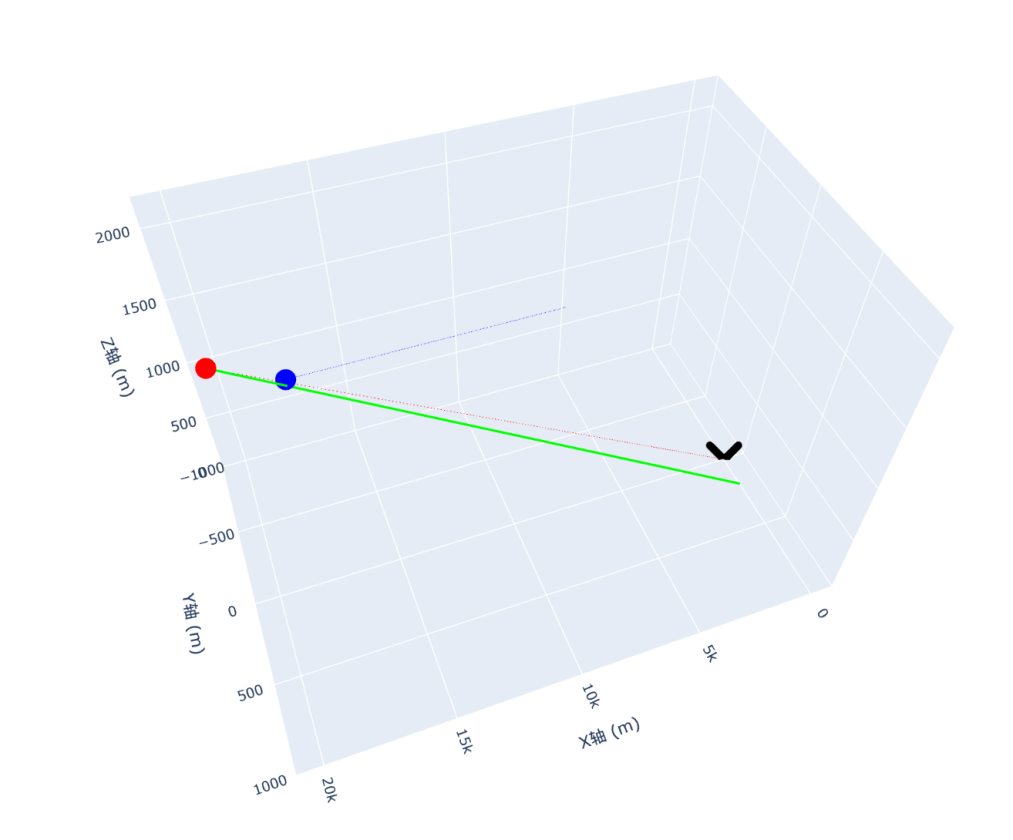
\includegraphics[width=0.5\textwidth]{pic/Fg1.png}
			\caption{空间坐标系与物体分布状态}
			\label{fig:spatial_distribution}
		\end{figure}
		
		在本模型中,假设无人机 FY1 在 $xOy$ 平面内以 $120 \, \mathrm{m/s}$ 的速度朝向假目标飞行,且飞行过程中高度保持不变。无人机在执行任务后 $t_d = 1.5 \, \mathrm{s}$ 时投放一枚烟幕干扰弹,该干扰弹在投放后 $t_{\text{delay}} = 3.6 \, \mathrm{s}$ 起爆。
		
		无人机的飞行速度方向由当前位置指向假目标原点 $\mathbf{O} = (0, 0, 0)$,其速度矢量可表示为:
		\begin{equation}
			\mathbf{v}_d = \frac{\mathbf{O} - \mathbf{P}_{d0}}{\| \mathbf{O} - \mathbf{P}_{d0} \|} \cdot v_d,
		\end{equation}
		其中 $v_d = 120 \, \mathrm{m/s}$。无人机飞行过程中保持高度不变,其速度矢量的 $z$ 分量为零。
		
		在 $t_d = 1.5 \, \mathrm{s}$ 时刻,无人机投放干扰弹,此时无人机的位置为干扰弹的初始位置:
		\begin{equation}
			\mathbf{P}_{\text{drop}} = \mathbf{P}_{d0} + \mathbf{v}_d \cdot t_d.
		\end{equation}
		
		干扰弹投放时的初速度与无人机的速度相同,即 $\mathbf{v}_d$。在起爆前,将干扰弹视为质点,并忽略空气阻力,其运动遵循平抛运动规律。设从投放时刻起经过时间 $\tau$,干扰弹的位置为:
		\begin{equation}
			\mathbf{P}_{\text{shell}}(\tau) = \mathbf{P}_{\text{drop}} + \mathbf{v}_d \cdot \tau + \frac{1}{2} (0, 0, -g) \tau^2,
		\end{equation}
		其中重力加速度取 $g = 9.8 \, \mathrm{m/s}^2$。
		
		干扰弹在投放后 $t_{\text{delay}} = 3.6 \, \mathrm{s}$ 时刻起爆,起爆点位置为:
		\begin{equation}
			\mathbf{P}_{\text{explode}} = \mathbf{P}_{\text{drop}} + \mathbf{v}_d \cdot t_{\text{delay}} + \frac{1}{2} (0, 0, -g) t_{\text{delay}}^2.
		\end{equation}
		
		起爆后瞬时形成一个半径为 $R_s = 10 \, \mathrm{m}$ 的球状烟幕云团,云团中心以 $v_s = 3 \, \mathrm{m/s}$ 的速度匀速垂直下沉。设从起爆时刻起经过时间 $t$,烟幕云团中心的位置为:
		\begin{equation}
			\mathbf{P}_{\text{smog}}(t) = \mathbf{P}_{\text{explode}} + (0, 0, -v_s \cdot t).
		\end{equation}
		
		烟幕云团在起爆后持续存在 $T_{\text{exist}} = 20 \, \mathrm{s}$,在此期间具备遮蔽能力。
		
		\subsubsection{导弹飞行的空间物理模型}
		
		将导弹 M1 视为质点,其从初始位置 $\mathbf{P}_{M1}(0)$ 以恒定速率 $v_m = 300 \, \mathrm{m/s}$ 沿直线飞向原点 $\mathbf{O}$。其速度矢量为:
		\begin{equation}
			\mathbf{v}_m = \frac{\mathbf{O} - \mathbf{P}_{M1}(0)}{\| \mathbf{O} - \mathbf{P}_{M1}(0) \|} \cdot v_m.
		\end{equation}
		
		在 $t \geq 0$ 时刻,导弹的位置可表示为:
		\begin{equation}
			\mathbf{P}_m(t) = \mathbf{P}_{M1}(0) + \mathbf{v}_m \cdot t.
		\end{equation}
		
		\subsubsection{有效遮蔽时间的确定}
		
		考虑真目标表面任意一点与导弹位置的连线构成一条线段。若在某一时刻,该线段与球状烟幕云团存在交点,则认为烟幕干扰弹在该时刻对该点实现了有效遮蔽。\cite{1}
		
		采用随机抽样方法,在真目标(圆柱体)表面均匀随机选取1000个点作为目标点集。目标的面积遮挡比反映了目标被烟幕遮挡的程度,可以用被烟幕遮蔽目标的面积与无烟幕干扰时目标的面积的比值进行度量。定义烟幕干扰度为 $D$,则:
		\begin{equation}
			D = \frac{S}{S_0}
		\end{equation}
		式中 $S$ 为目标被烟幕遮挡区域的面积,$S_0$ 为无烟幕干扰时目标的面积。
		
		当烟幕对目标的面积遮挡比发生变化时,导引头对目标的识别准确度也随之变化\cite{2}。当烟幕遮挡面积比小于70\% 时,目标具备抗烟幕干扰能力,且随着遮挡面积比的增加,识别概率不断下降\cite{3}。故本文采用70\%的烟幕面积遮挡比作为识别目标的临界值。
		
		记在时刻$t$,连接导弹位置与各目标点所得线段中,与烟幕云团存在公共点的点数为有效遮蔽点数。通过计算$t$时刻下有效遮蔽点数与总目标点数的比值$R(t)$并与70\%进行对比,即可判断烟幕干扰弹在该时刻对真目标实现了有效遮蔽。若$R(t)>0.7$,则认为该时刻满足有效遮蔽条件。
		
		\subsubsection{求解流程及结果}
		
		采用步进法进行时间推进,时间步长设为$\Delta t = 0.001\,\mathrm{s}$。在每一时间步内,依次判断每个目标点与导弹连线是否与球状烟幕云团相交,统计有效遮蔽点数并计算$R(t)$。
		
		总有效遮蔽时间通过累加所有满足$R(t)$大于一定阈值的时间步长获得,其时间积分精度由步长$\Delta t$决定,即最小分辨时间为$0.001\,\mathrm{s}$。
		
		本次求解流程中,通过设置不同的烟幕干扰度判断阈值,求解出不同结果。
		
		求解流程图如图\ref{fig:flowchart_q1}所示:
		
		\begin{figure}[H]
			\centering
			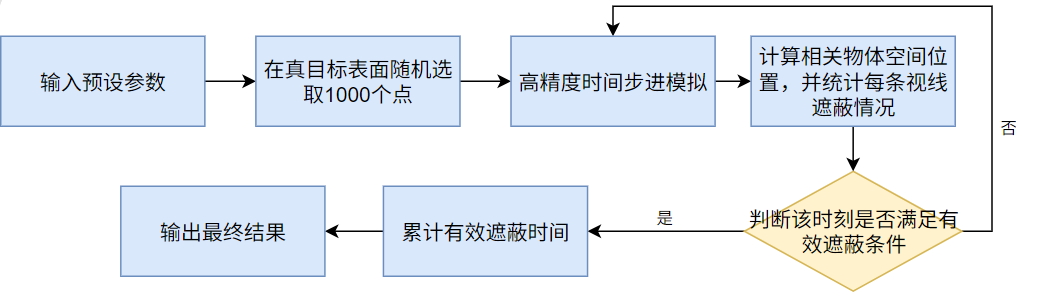
\includegraphics[width=0.8\textwidth]{pic/Fg2.png}
			\caption{问题一求解流程图}
			\label{fig:flowchart_q1}
		\end{figure}
		
		程序模拟结果如下表所示:
		
		\begin{table}[H]
			\centering
			\caption{问题一:不同判断阈值下的有效遮蔽时长(单位:秒)}
			\label{tab:results_q1}
			\begin{tabular}{cccccccccccc}
				\toprule
				\textbf{判断阈值 (\%)} & \textbf{100} & \textbf{90} & \textbf{80} & \textbf{70} & \textbf{60} & \textbf{50} & \textbf{40} & \textbf{30} & \textbf{20} & \textbf{10} \\
				\midrule
				\textbf{有效遮蔽时长 (s)} & 1.393 & 1.406 & 1.413 & 1.420 & 1.428 & 1.436 & 1.444 & 1.452 & 1.459 & 1.468 \\
				\bottomrule
			\end{tabular}
		\end{table}
		
		选取70\%的烟幕面积遮挡比作为识别目标的临界值时,烟幕干扰弹的有效遮蔽时长为$1.420\,\mathrm{s}$。通过程序模拟动画进一步验证,其演示结果如图\ref{fig:simulation_q1}所示。
		
		\begin{figure}[H]
			\centering
			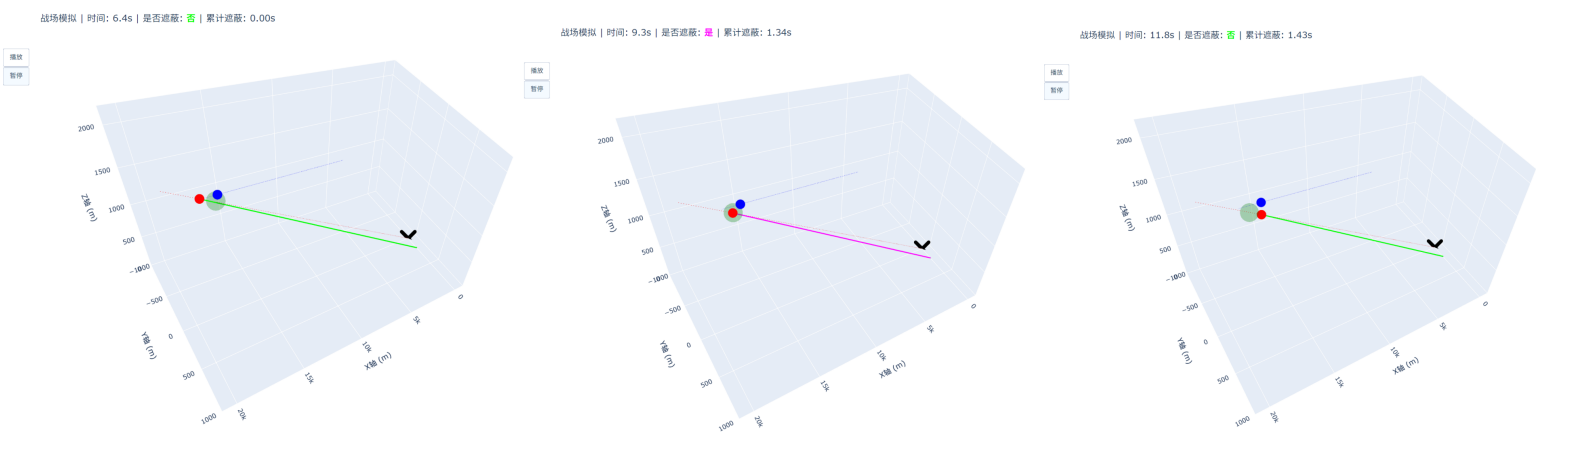
\includegraphics[width=0.8\textwidth]{pic/Fg3.png}
			\caption{问题一程序模拟动画关键帧}
			\label{fig:simulation_q1}
		\end{figure}
		
		可以看出,程序求解结果正确。当无人机运动与投弹情况满足问题一题设参数时,烟幕干扰弹的有效遮蔽时长为$1.420\,\mathrm{s}$。
		
		
		\subsection{问题二的模型建立与求解}
		
		针对问题二,决策目标是确定无人机FY1的最优飞行与投放策略,以最大化单枚烟幕弹对M1导弹的有效遮蔽时长。为解决这个非凸优化问题,设计了一个鲁棒性强的\textbf{"全局粗搜 $\rightarrow$ 局部精调 $\rightarrow$ 精细测算"}三阶段优化框架。该框架通过系统性的搜索与迭代,高效地在广阔的解空间中定位全局最优解或其高质量近似解\cite{4}。
		
		\subsubsection{决策变量与目标函数}
		
		\begin{enumerate}
			\item \textbf{决策变量}: 该模型需要优化四个关键参数来定义无人机的完整策略:
			
			- 无人机飞行速度 $v$ (m/s)\\
			\indent	- 无人机飞行方向 $\theta$ (弧度)\\
			\indent	- 烟幕弹投放时间 $t_{\text{drop}}$ (s)\\
			\indent	- 烟幕弹引信延迟时间 $t_{\text{delay}}$ (s)
			
			\item \textbf{约束条件}:
			\begin{align}
				\left\{
				\begin{aligned}
					\text{无人机速度约束:} &\quad 70 \le v \le 140\,\text{m/s} \\
					\text{物理可行性约束:} &\quad t_{\text{drop}} > 0,\quad t_{\text{delay}} > 0
				\end{aligned}
				\right.
			\end{align}
			
			\item \textbf{目标函数}: 该模型核心目标是最大化最终的有效遮蔽时间 $T_{\text{occlusion}}$。
			\begin{equation}
				\max T_{\text{occlusion}}(v, \theta, t_{\text{drop}}, t_{\text{delay}})
			\end{equation}
		\end{enumerate}
		
		\subsubsection{三阶段优化框架}
		
		\paragraph{第一阶段:全局粗搜与可行解窗口定位}
		此阶段的目标是在整个解空间中快速、广泛地识别出具有潜力的"可行解窗口",为后续的精细优化提供高质量的起点。本研究创新性地采用了\textbf{逆向建模}的思路。
		
		如图\ref{fig:flowchart_q2}左侧所示,首先离散化烟幕起爆时间 $t_{\text{explode}}$ 和起爆点在初始导弹-目标视线上的相对位置比例 $los\_ratio$。对于每一个 $(t_{\text{explode}}, t_{\text{delay}}, los\_ratio)$ 组合,可以反向推算出唯一确定的理想起爆点坐标 $P_{\text{explode}}$。
		
		基于 $P_{\text{explode}}$ 和投放延迟 $t_{\text{delay}}$,可以解析出无人机为了实现此次爆炸所\textbf{必须具备}的三维速度矢量 $\vec{V}_{\text{UAV, required}}$。其计算公式如下:
		\begin{equation}
			P_{\text{explode}} = P_{\text{UAV,initial}} + \vec{V}_{\text{UAV, required}} \cdot t_{\text{explode}} + \frac{1}{2} \vec{g} \cdot t_{\text{delay}}^2
		\end{equation}
		\begin{equation}
			\vec{V}_{\text{UAV, required}} = \frac{P_{\text{explode}} - P_{\text{UAV,initial}} - (0, 0, -0.5gt_{\text{delay}}^2)}{t_{\text{explode}}}
		\end{equation}
		
		随后,需要对该速度进行可行性剪枝:检查其水平分量的模长(即无人机速度 $v$)是否在 $[70, 140]$ m/s 的区间内。通过此方法高效地过滤掉大量不可行解。对于每个可行策略,首先使用简化的目标模型(将真目标视为一个质点)快速计算其遮蔽时长。最终,从数百万个搜索点中筛选出数万个可行解,并选取其中遮蔽时长最长且分布稀疏的500个解作为第二阶段的优化起点。
		
		\paragraph{第二阶段:多起点局部精调}
		此阶段的目标是从这些高质量的起点出发,进行精细的局部寻优。
		采用\textbf{坐标上升法}作为局部优化算法,其迭代过程如图\ref{fig:flowchart_q2}中部所示。该算法在每次迭代中,会依次固定其他三个决策变量,仅对其中一个变量在其邻域内进行一维搜索,以找到能使目标函数最大化的值。具体来说,对于当前最优参数 $(v, \theta, t_{\text{drop}}, t_{\text{delay}})$,依次在以下区间内进行线性搜索:
		
		- $v_{\text{new}} \in [v-5, v+5]$\\
		\indent	- $\theta_{\text{new}} \in [\theta-10^\circ, \theta+10^\circ]$\\
		\indent	- $t_{\text{drop, new}} \in [t_{\text{drop}}-1, t_{\text{drop}}+1]$\\
		\indent	- $t_{\text{delay, new}} \in [t_{\text{delay}}-1, t_{\text{delay}}+1]$
		
		重复此过程直至目标函数值不再有显著提升(收敛阈值设为0.001s)或达到最大迭代次数(10次)。流程图中的判断环节确保算法在满足收敛条件时及时停止迭代。
		
		\paragraph{第三阶段:高精度模型测算}
		为了得到最终的精确遮蔽时间,使用最高精度的模型对第二阶段输出的全局最优候选解进行最终测算,如图\ref{fig:flowchart_q2}右侧所示。此阶段与前两阶段的核心区别在于对\textbf{真目标的建模方式},需要考虑真目标的实际几何形状。
		
		在圆柱形的真目标表面随机均匀采样1000个点,在每个仿真时间步(0.001s),我们判断这1000条从导弹位置到目标采样点的视线中,被烟幕球体遮挡的比例。累计所有有效遮蔽的时间步,便得到最终的高精度遮蔽时长。
		
		图\ref{fig:flowchart_q2}展示了完整的求解流程,清晰地呈现了三个优化阶段之间的逻辑关系和迭代过程。该流程从全局解空间出发,通过逆向建模快速定位可行解窗口,再通过坐标上升法进行局部精调,最终通过高精度测算获得最优解。
		
		
		\begin{figure}[H]
			\centering
			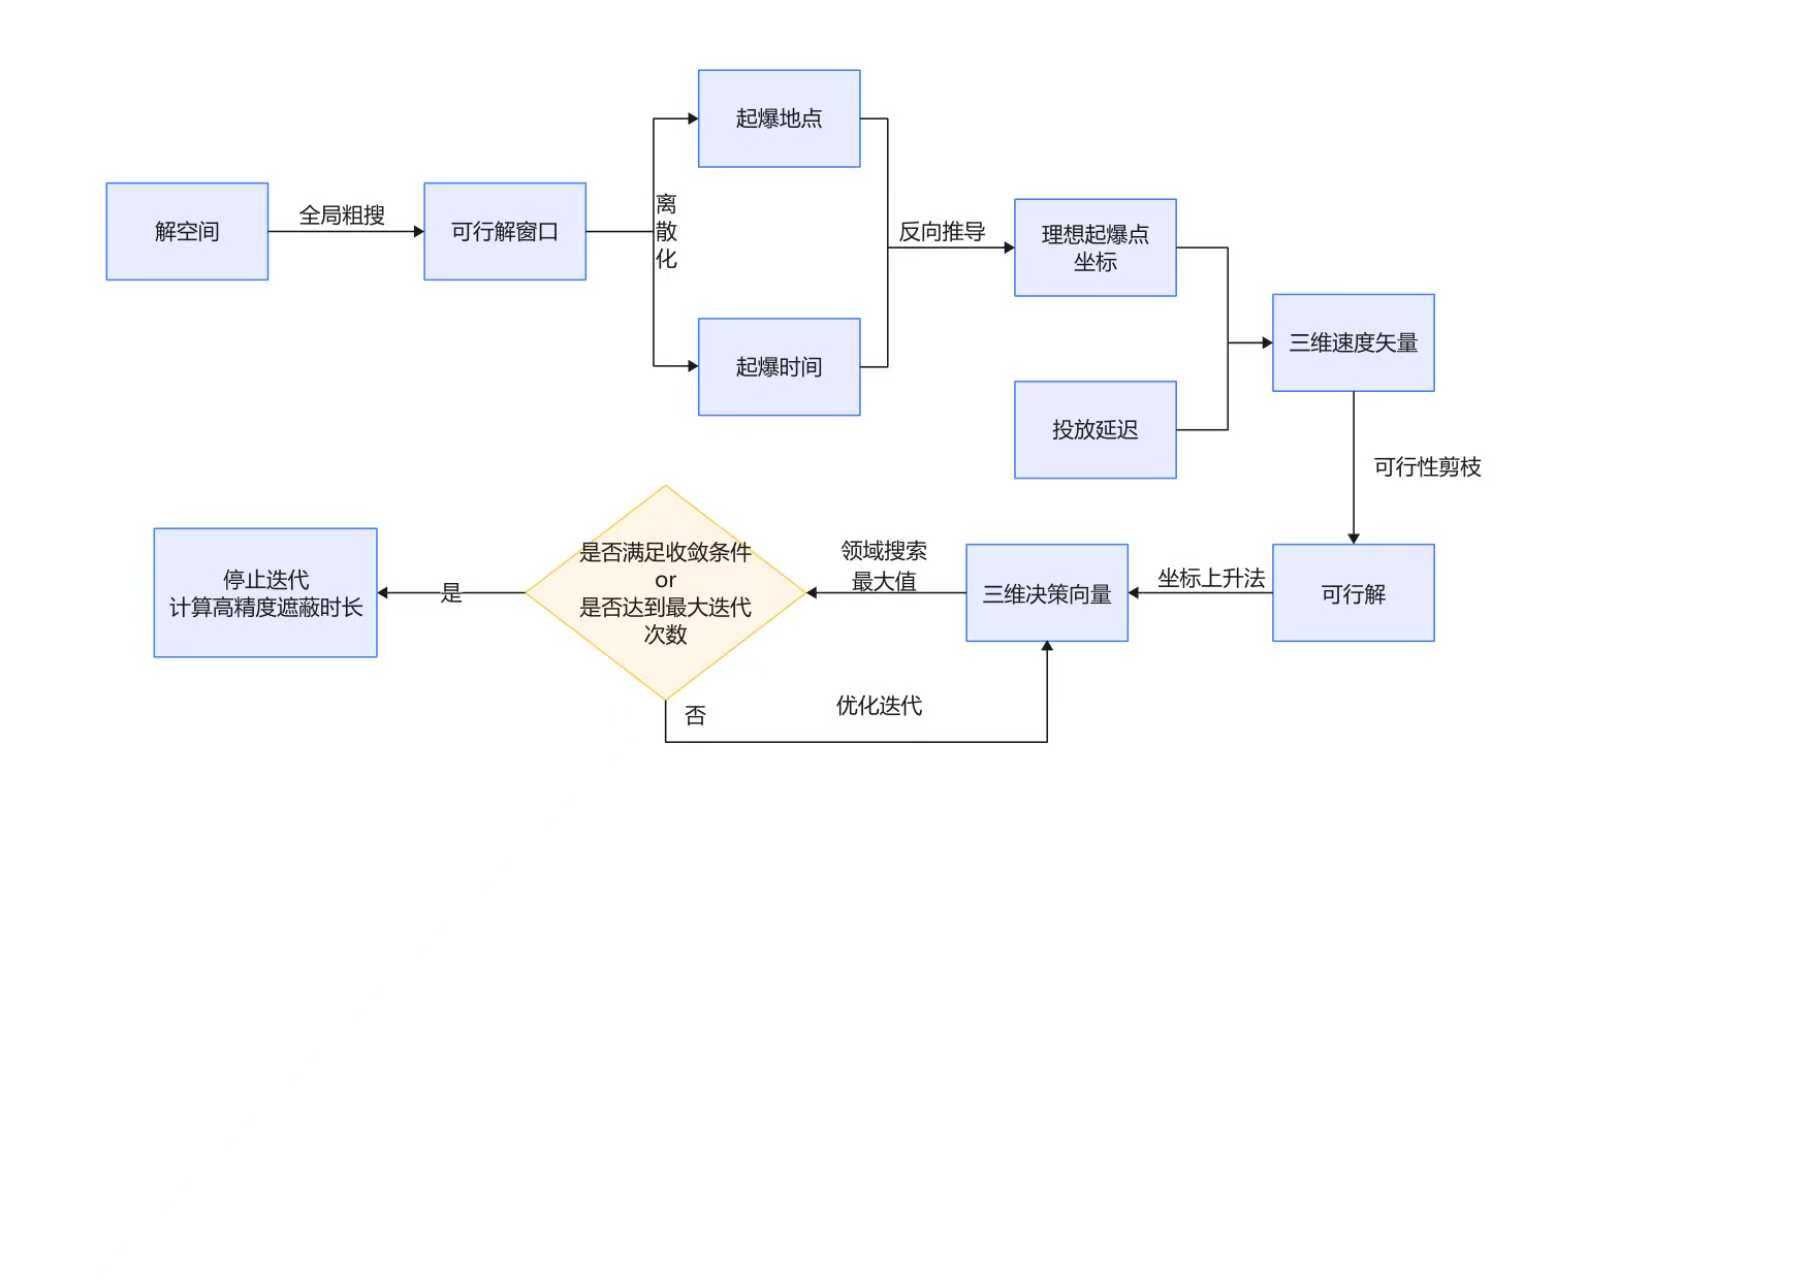
\includegraphics[width=0.8\textwidth]{pic/Fg6-Pb2.jpg}
			\caption{问题二求解流程图}
			\label{fig:flowchart_q2}
		\end{figure}
		
		\subsubsection{模型求解}
		\begin{enumerate}
			\item \textbf{全局粗搜求解}: 对起爆时间、引信延迟和视线比率进行大范围离散化搜索,并调用\code{check\_reachability}函数进行可行性判断,最终获得500个高质量的初始解。
			
			\item \textbf{局部精调求解}: 对这500个初始解执行\code{step2\_local\_optimization}函数进行坐标上升优化。图\ref{fig:pca_q2_left}展示了优化过程中目标函数(遮蔽时长)的收敛情况。从图中可以看出我们的坐标上升算法非常高效,通常在短短几次迭代内就能收敛。
			
			\item \textbf{结果与分析}: 在500个局部最优点中,选取了遮蔽时长最长的解作为全局最优候选解。图\ref{fig:pca_q2_right}直观展示了从初始解到最终局部最优解的变化过程。初始解(蓝点)广泛分布,经过优化后(箭头方向),它们收敛至多个不同的区域(红点簇),这有力地证明了该问题的非凸性,并凸显了我们采用\textbf{多起点优化}策略的必要性和正确性,极大地降低了模型陷入较差局部最优解的风险。最终选出全局最佳候选解(绿色星标)。整个求解过程充分体现了流程图中所展示的系统性和完整性。
			
			\begin{figure}[H]
				\centering
				\begin{minipage}[b]{0.48\textwidth}
					\centering
					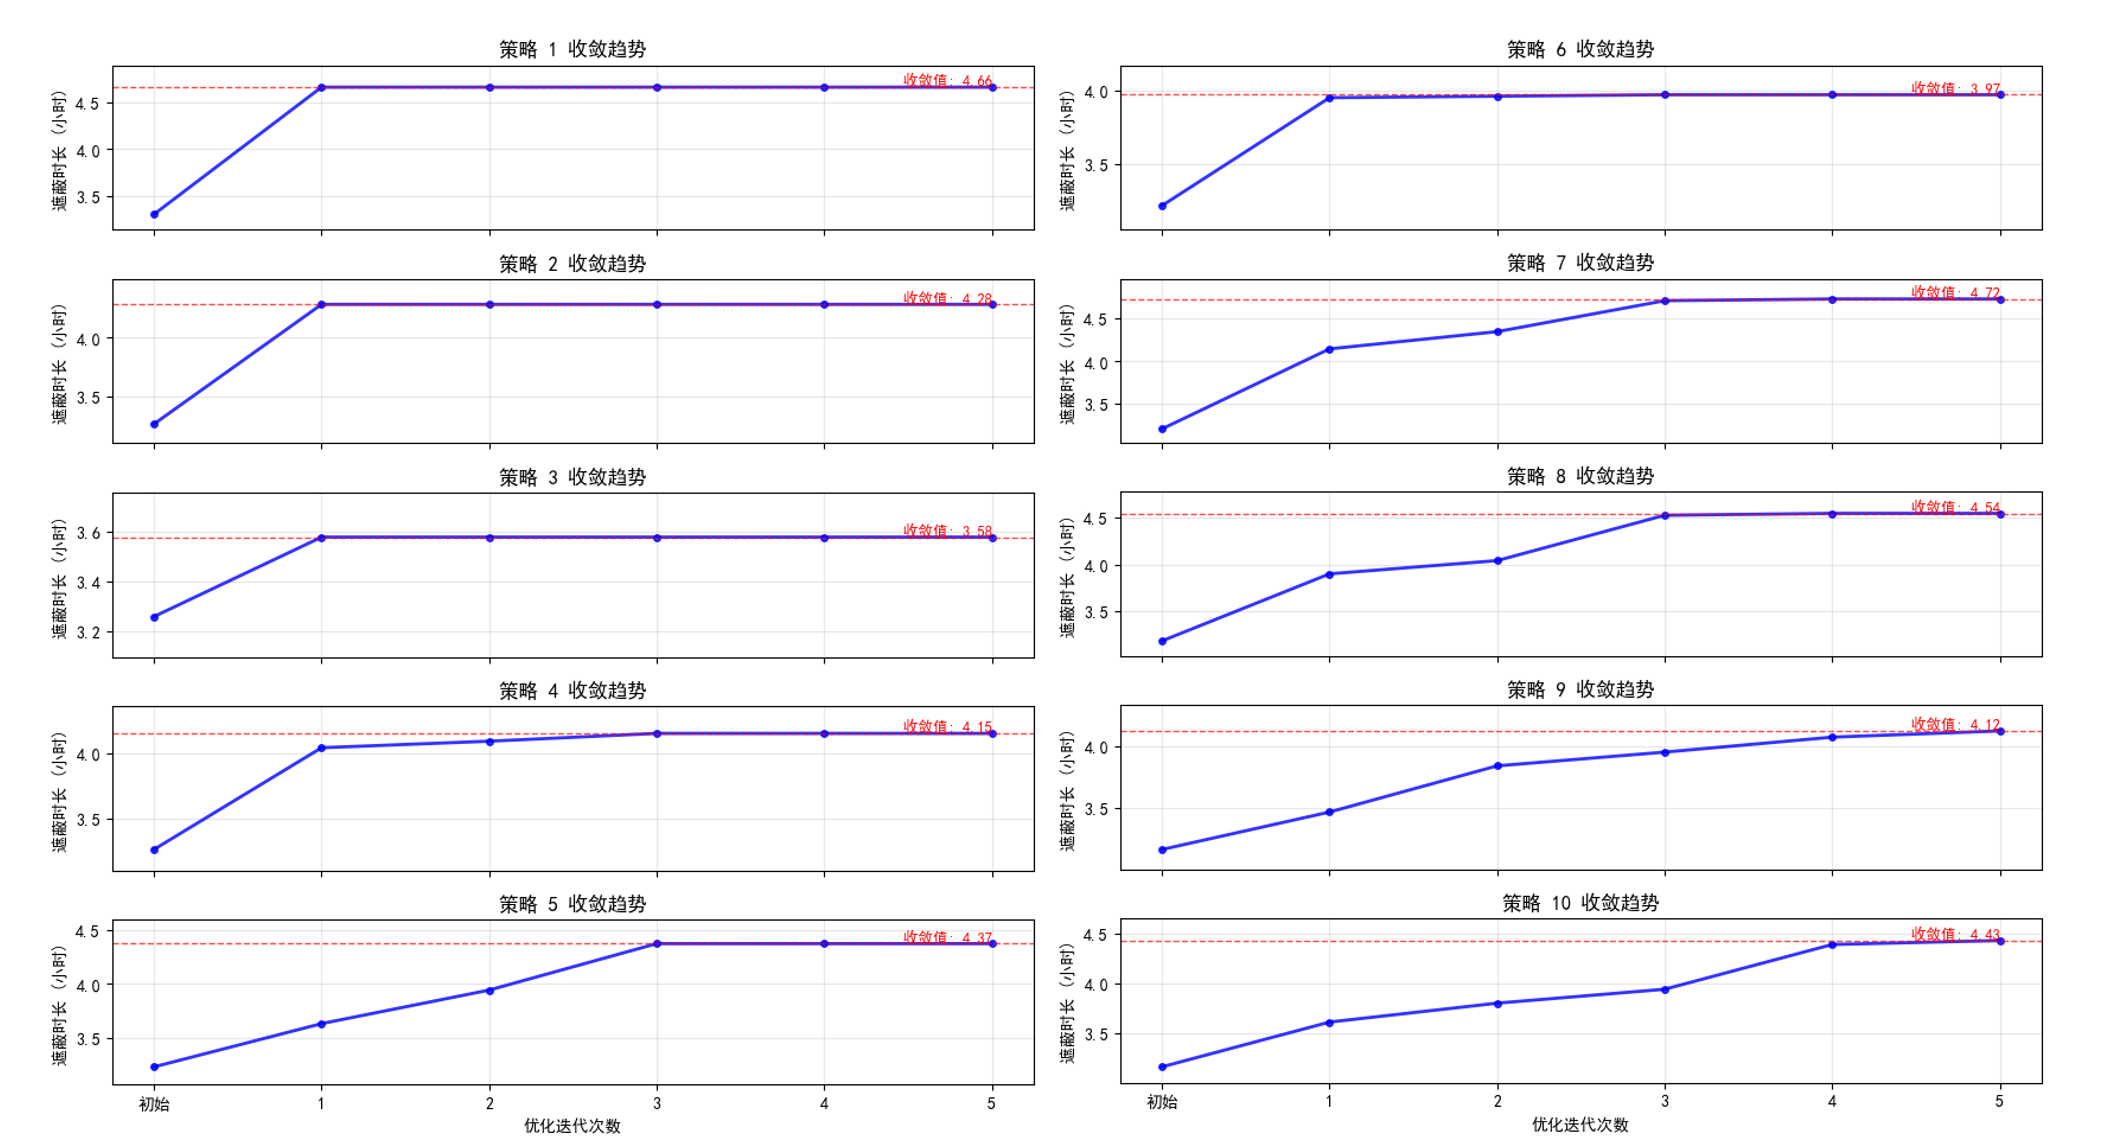
\includegraphics[width=\textwidth, height=0.25\textheight]{pic/Fg4.png}
					\caption{目标函数(遮蔽时长)的收敛情况}
					\label{fig:pca_q2_left}
				\end{minipage}
				\hfill
				\begin{minipage}[b]{0.48\textwidth}
					\centering
					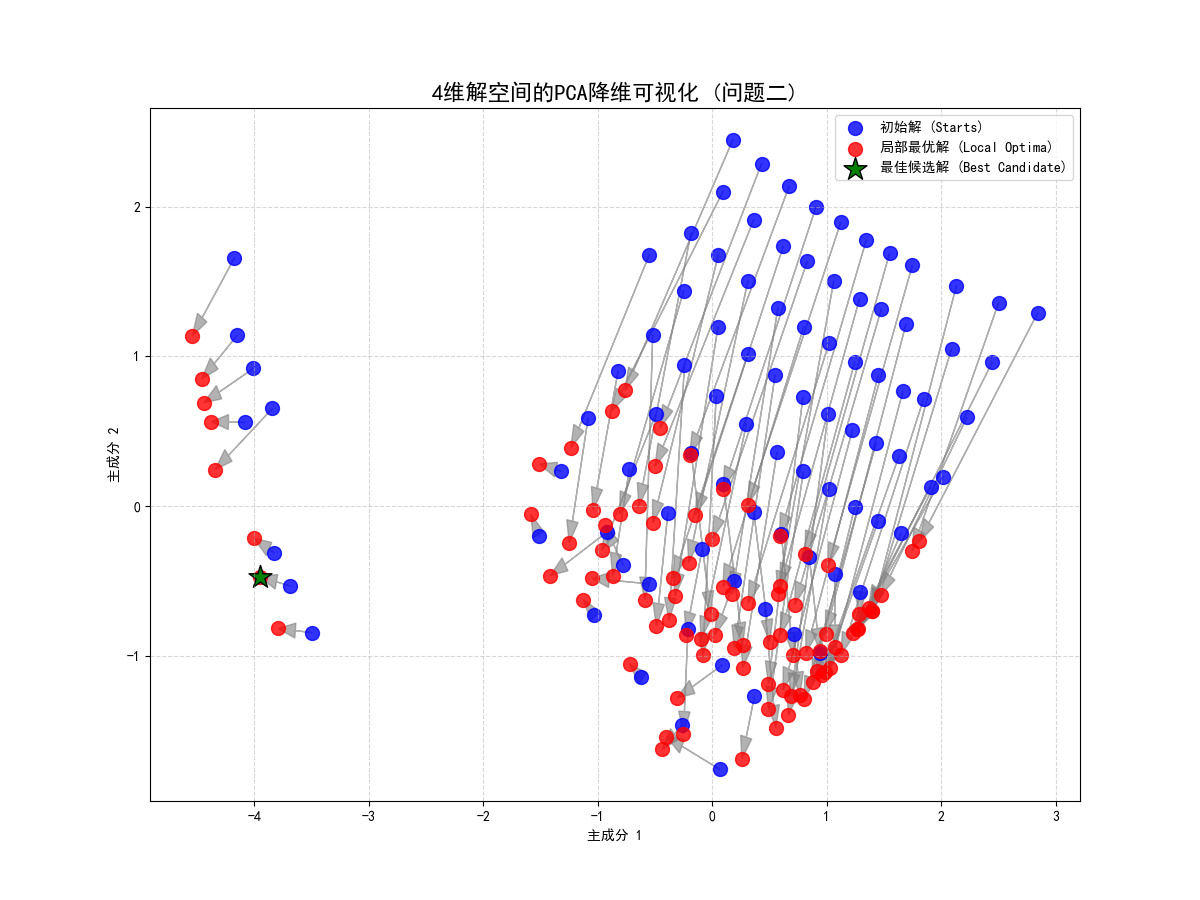
\includegraphics[width=\textwidth, height=0.25\textheight]{pic/Fg5.png}
					\caption{坐标上升法求解过程}
					\label{fig:pca_q2_right}
				\end{minipage}
			\end{figure}
			
			\item \textbf{最终测算}: 将最佳候选解输入\code{step3\_final\_validation}函数进行高精度测算,得到最终的优化结果,如表\ref{tab:results_q2}所示。
		\end{enumerate}
		
		% --- 插入您的Q2结果表格 ---
		\begin{table}[H]
			\centering
			\caption{问题二:最优策略与结果}
			\label{tab:results_q2}
			\begin{tabular}{@{}lcc@{}}
				\toprule
				决策变量               & 最优值      & 单位 \\ \midrule
				无人机飞行速度 ($v$)     & 77.4556 & m/s  \\
				无人机飞行方向 ($\theta$)    & 178.2870  & 度   \\
				烟幕弹投放时间 ($t_{\text{drop}}$) & 0.3455 & 秒   \\
				引信延迟时间 ($t_{\text{delay}}$)   & 2.6846 & 秒   \\ \midrule
				\textbf{最终高精度遮蔽时长} & \textbf{4.6160} & \textbf{秒}   \\ \bottomrule
			\end{tabular}
		\end{table}
		
		\begin{figure}[H]
			\centering
			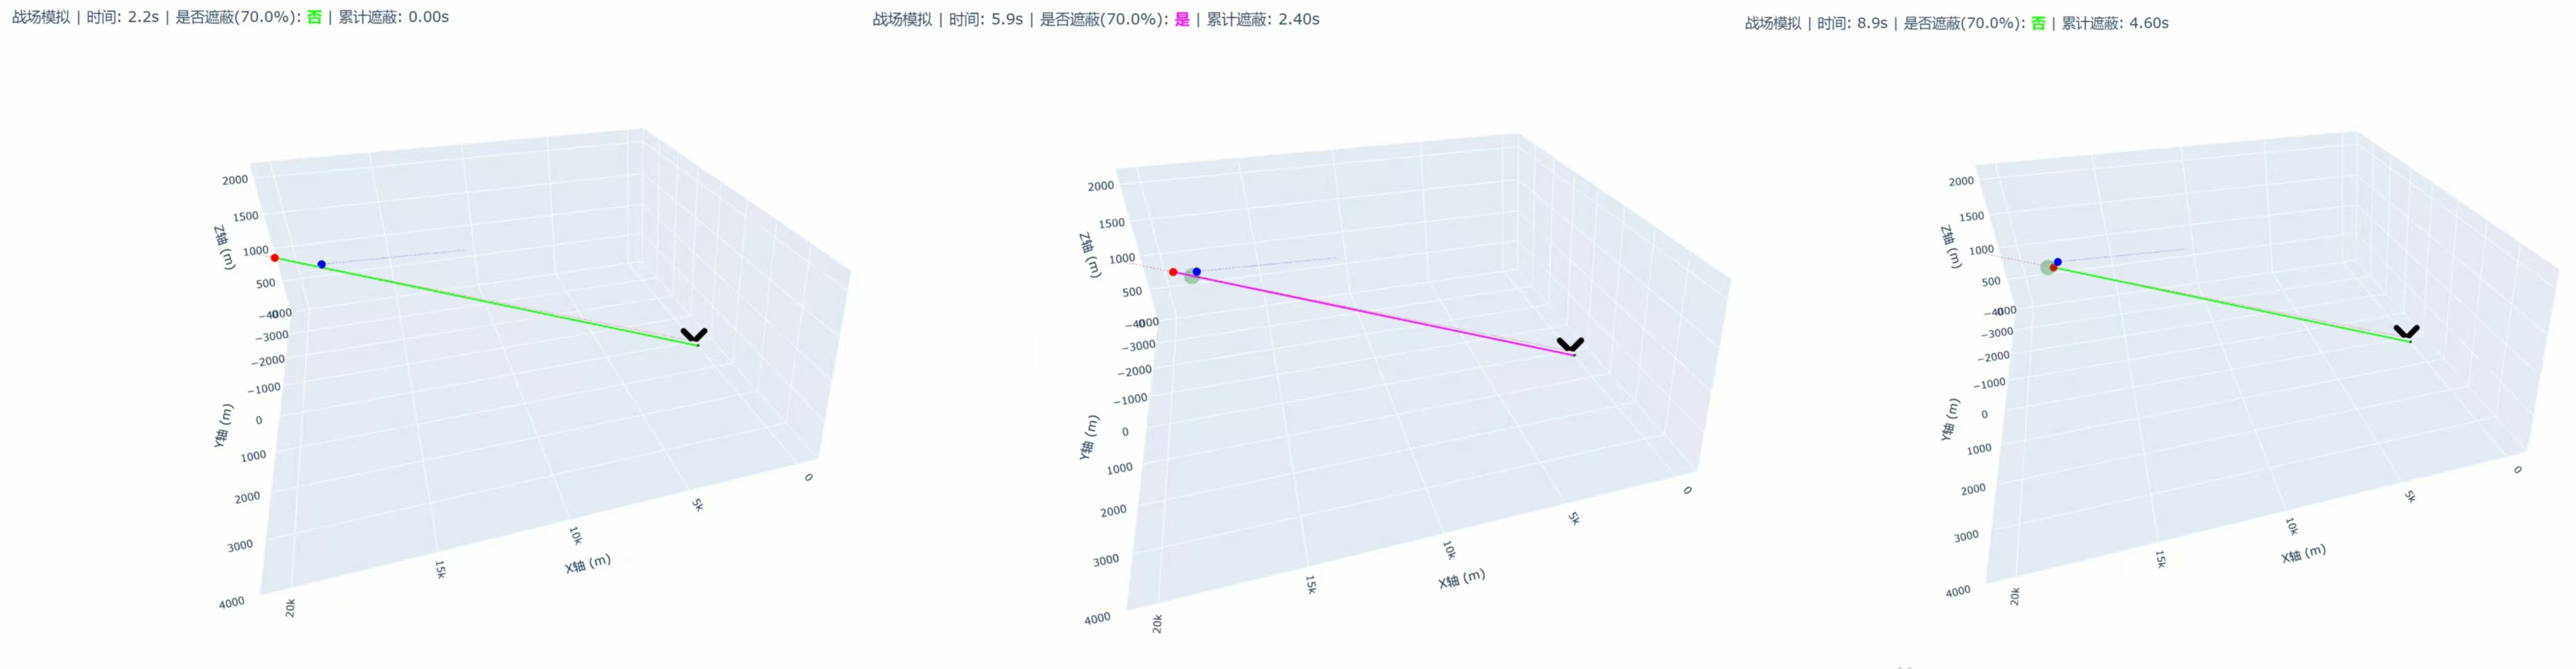
\includegraphics[width=0.8\textwidth]{pic/sim2.jpg}
			\caption{问题二程序模拟动画关键帧}
			\label{fig:simulation_q2}
		\end{figure}
		
		\subsection{问题三的模型建立与求解}
		
		问题三要求使用无人机FY1投放三枚烟幕弹对M1进行干扰。这使得问题从单点决策演变为\textbf{多目标协同优化},本研究在问题二成功的三阶段优化框架基础上,对其进行了针对性的扩展和升级。
		
		\subsubsection{决策变量与目标函数的演进}
		
		\begin{enumerate}
			\item \textbf{决策变量扩展}: 无人机保持统一的飞行速度 $v$ 和方向 $\theta$。决策变量从4个扩展到8个,以控制三枚烟幕弹的投放:
			
			- $v, \theta$\\
			\indent - 第一枚弹的投放与延迟时间 $(t_{\text{drop1}}, t_{\text{delay1}})$\\
			\indent - 第二枚弹的投放与延迟时间 $(t_{\text{drop2}}, t_{\text{delay2}})$\\
			\indent - 第三枚弹的投放与延迟时间 $(t_{\text{drop3}}, t_{\text{delay3}})$
			
			\item \textbf{约束条件更新}: 新增了投放间隔约束,即
			\begin{equation}
				t_{\text{drop}(i+1)} - t_{\text{drop}(i)} \ge 1.0 s
			\end{equation}
			
			\item \textbf{目标函数升级——协同效应建模}:
			为准确评估三枚弹的\textbf{协同效应},本研究将目标函数 $T_{\text{total\_occlusion}}$ 定义为\textbf{三个遮蔽时间区间的并集总长度}。在数值仿真中,在每个时间步检查是否有\textbf{至少一个}烟幕云团正在提供有效遮蔽。这个新的目标函数能够正确地奖励那些通过时序配合来最大化总覆盖时间的策略。
			\begin{equation}
				T_{\text{total\_occlusion}} = \text{length} \left( \bigcup_{i=1}^{3} \text{OcclusionInterval}_i \right)
			\end{equation}
			
		\end{enumerate}
		
		\subsubsection{优化框架的适应性改进}
		继续沿用“全局粗搜-局部精调-精细测算”的宏观框架,但对核心模块进行了必要升级:
		
		\paragraph{第一阶段:全局粗搜} 保持不变。仍然通过对单枚烟幕弹的逆向建模来快速找到500个高质量的初始“锚点”。
		
		\paragraph{第二阶段:局部精调} 这是模型改进的核心。\\
		\indent - \textbf{初始化}: 将第一阶段得到的每个单弹策略 $(v, \theta, t_{\text{drop}}, t_{\text{delay}})$ 作为“种子”,生成一个初始的八维决策向量。例如,以该策略为中心弹,前后各布置一枚,形成 $(t_{\text{drop}}-1.2, t_{\text{delay}})$, $(t_{\text{drop}}, t_{\text{delay}})$, $(t_{\text{drop}}+1.2, t_{\text{delay}})$ 的初始投放序列。\\
		\indent - \textbf{高维坐标上升}: 将坐标上升法应用到新的8维决策空间中,在每次迭代中依次对8个变量进行一维邻域搜索。
		
		\paragraph{第三阶段:精细测算} 验证模型 \code{step3\_final\_validation\_multi} 被相应地修改,以同时模拟三个烟幕云团的运动和遮蔽效果,并根据新的协同目标函数计算最终的高精度总遮蔽时长。
		
		图\ref{fig:flowchart_q3}展示了问题三的完整的求解流程。
		
		
		\begin{figure}[H]
			\centering
			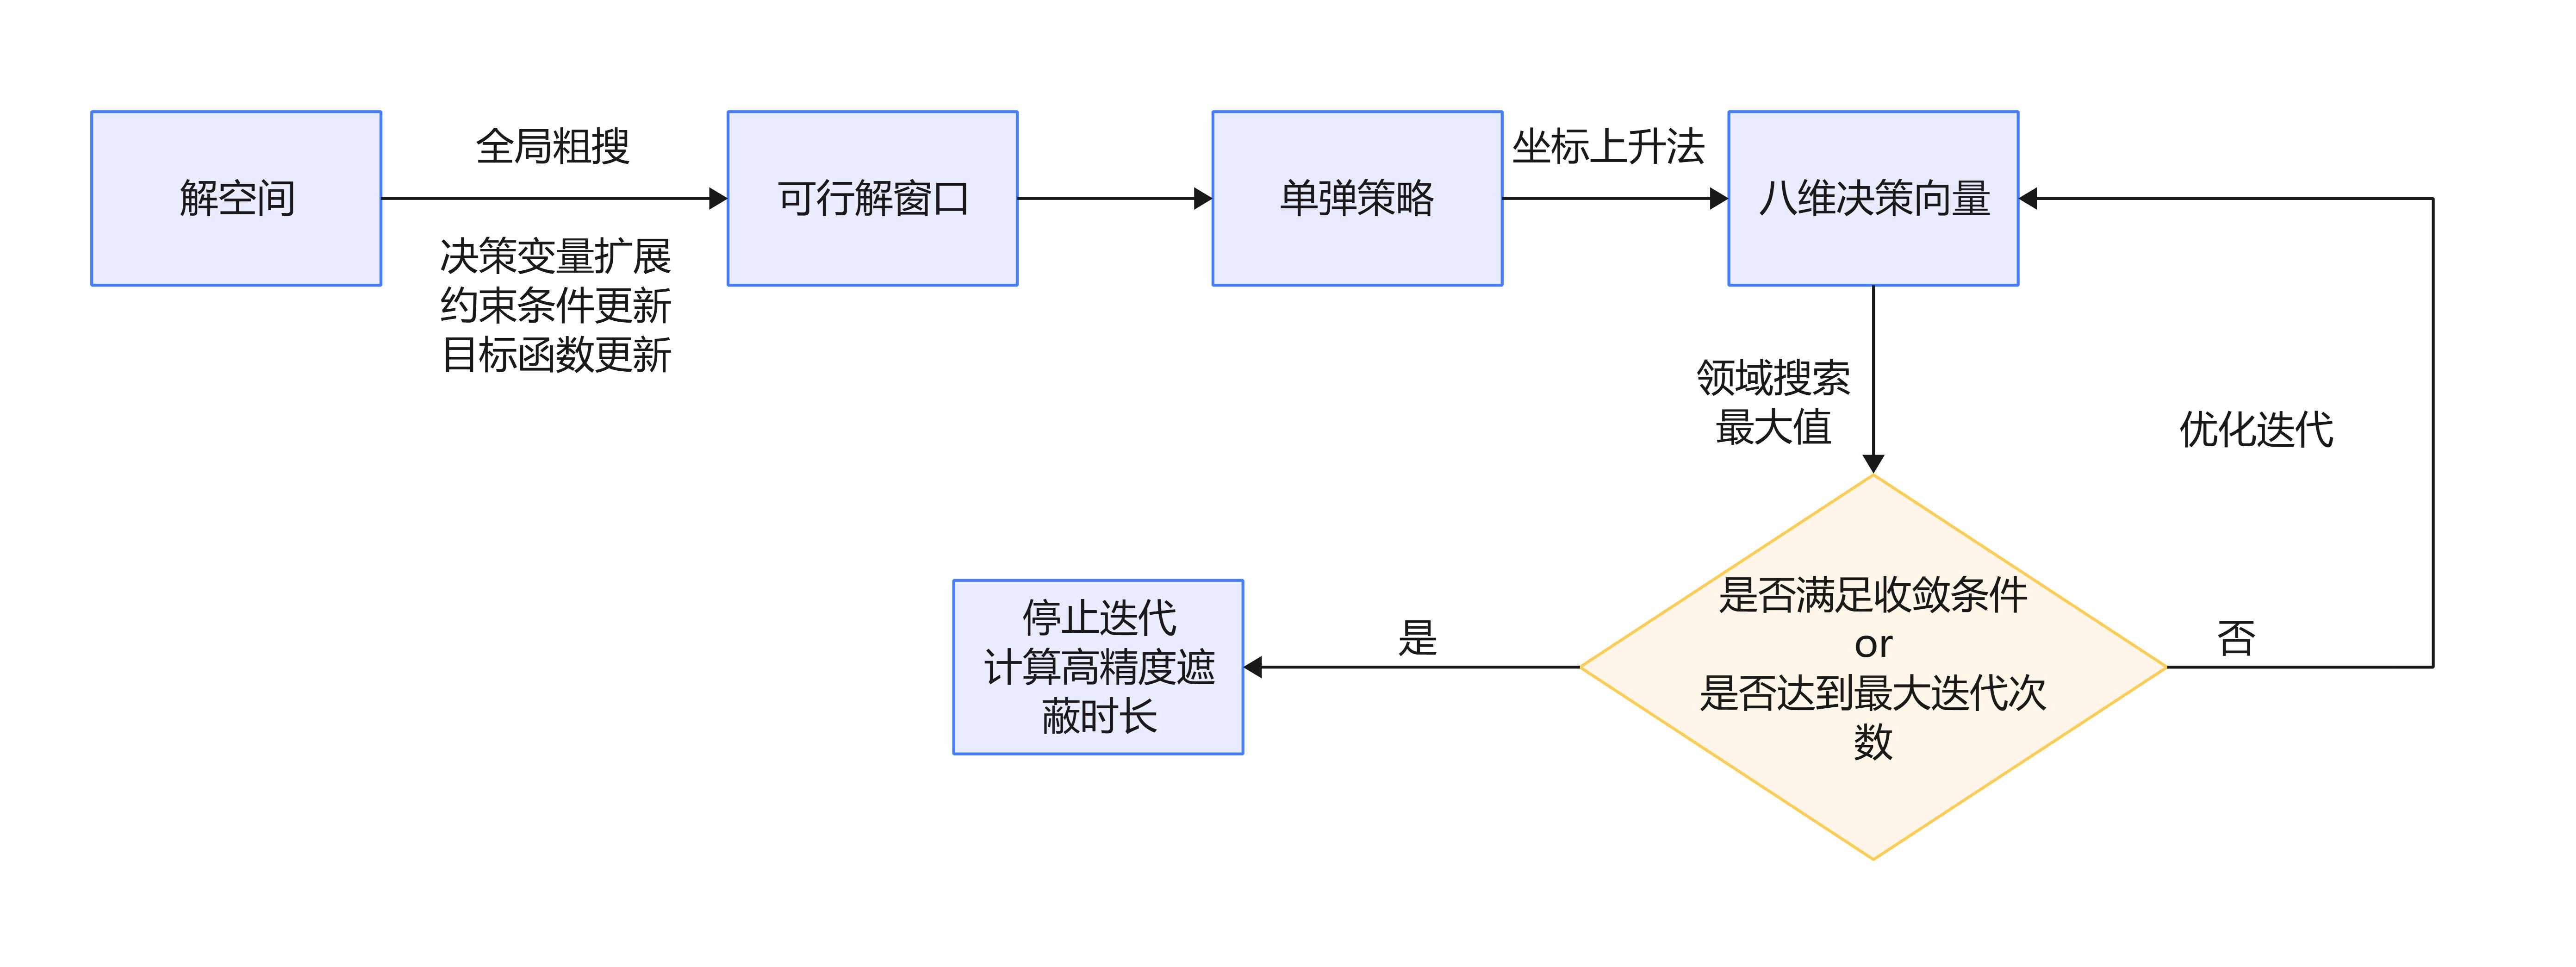
\includegraphics[width=0.8\textwidth]{pic/Fg7-Pb3.jpg}
			\caption{问题二求解流程图}
			\label{fig:flowchart_q3}
		\end{figure}
		
		\subsubsection{模型求解}
		\begin{enumerate}
			\item \textbf{求解流程}: 首先运行问题二的第一阶段代码,获得500个单弹初始解。随后,将每个解扩展为三弹初始策略,并输入升级后的\code{step2\_local\_optimization\_multi}\\函数进行高维局部优化。
			
			\item \textbf{结果与分析}: 最终从500个优化后的局部最优解中,选出使协同遮蔽时间最长的全局最优候选解。如图\ref{fig:pca_q3_left}、图\ref{fig:pca_q3_right}所示,尽管解空间维度翻倍,本项多起点优化算法依然表现出色,有效地探索了高维空间,并从多个初始点(蓝点)出发,最终收敛到不同的局部最优区域(红点)。
			
			\begin{figure}[H]
				\centering
				\begin{minipage}[b]{0.48\textwidth}
					\centering
					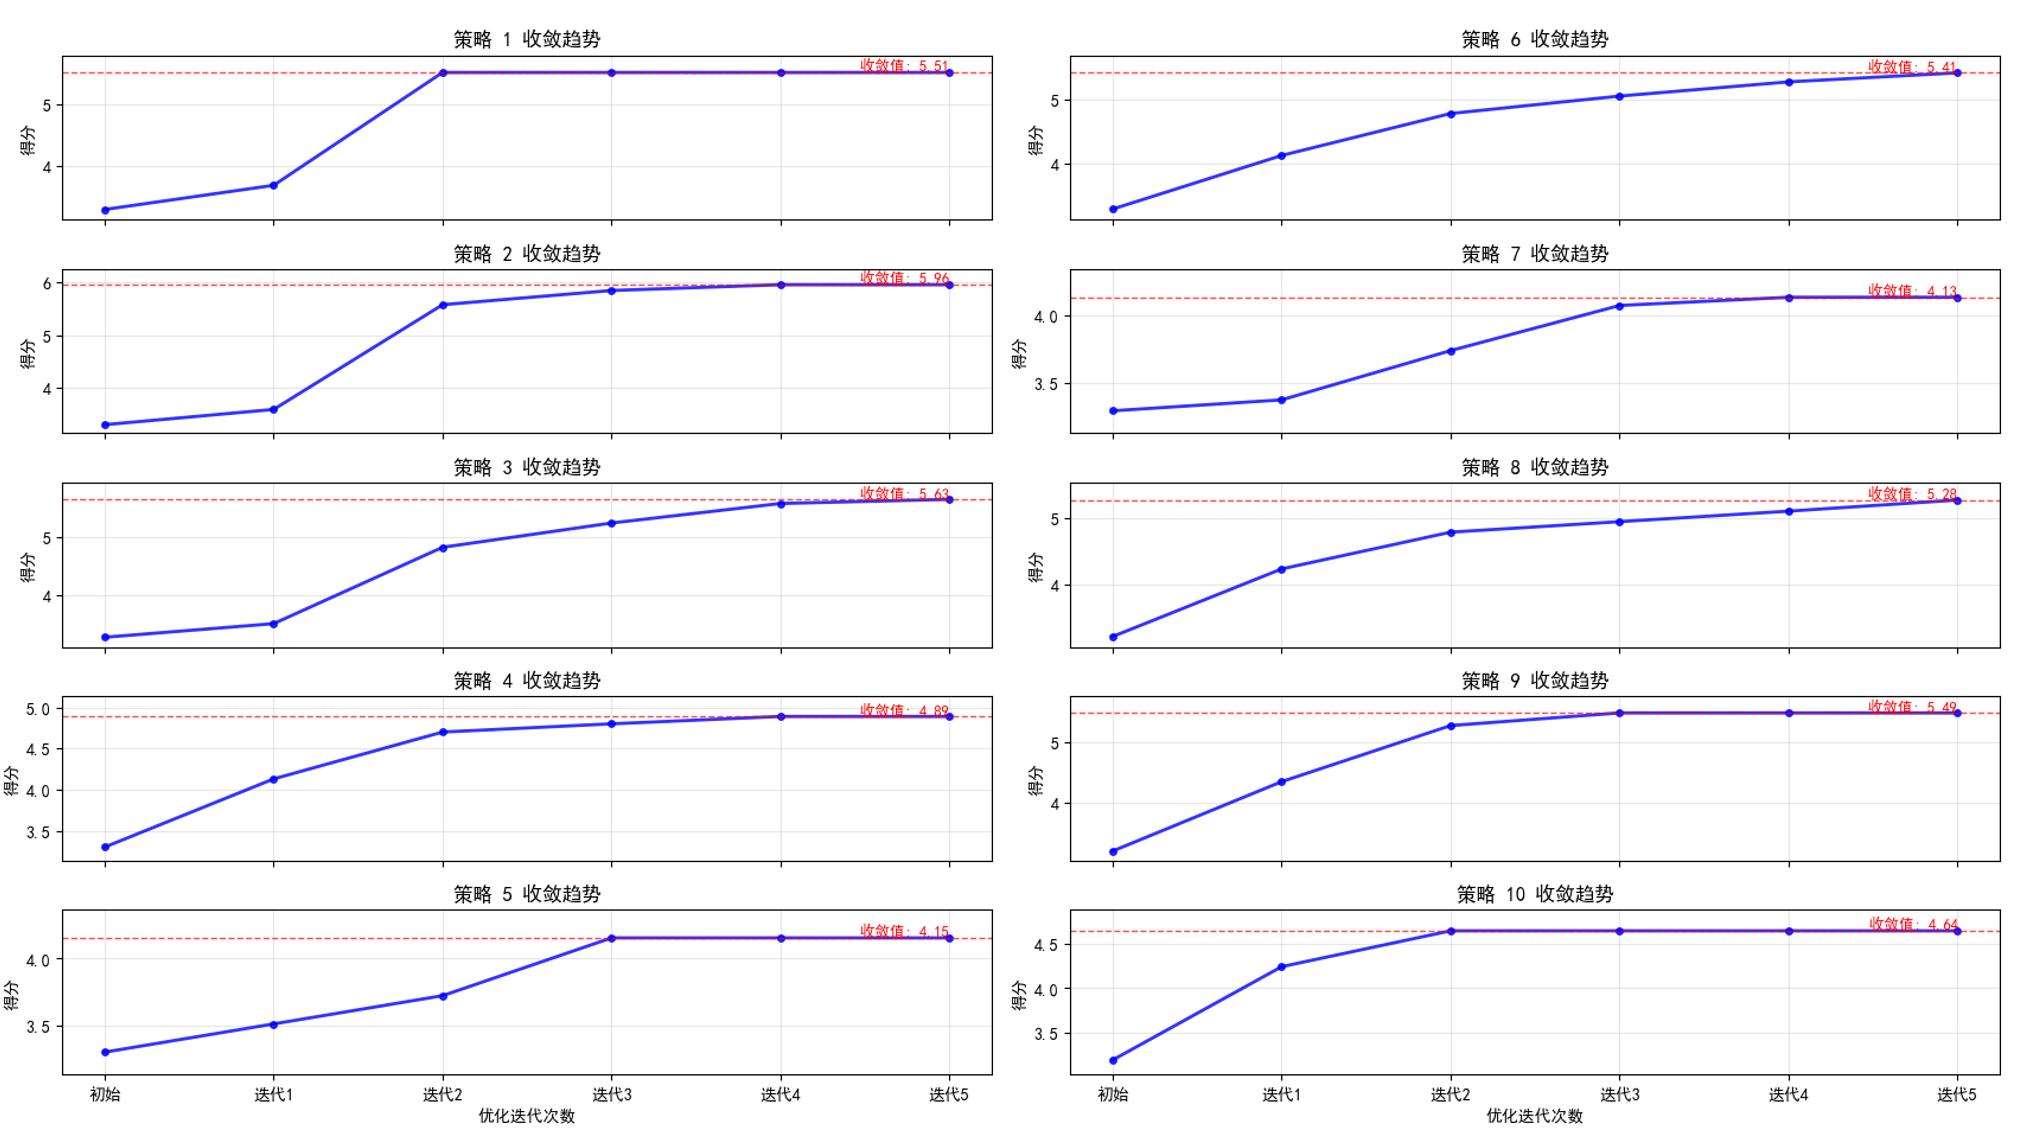
\includegraphics[width=\textwidth, height=0.25\textheight]{pic/Fg10.png}
					\caption{目标函数(遮蔽时长)的收敛情况}
					\label{fig:pca_q3_left}
				\end{minipage}
				\hfill
				\begin{minipage}[b]{0.48\textwidth}
					\centering					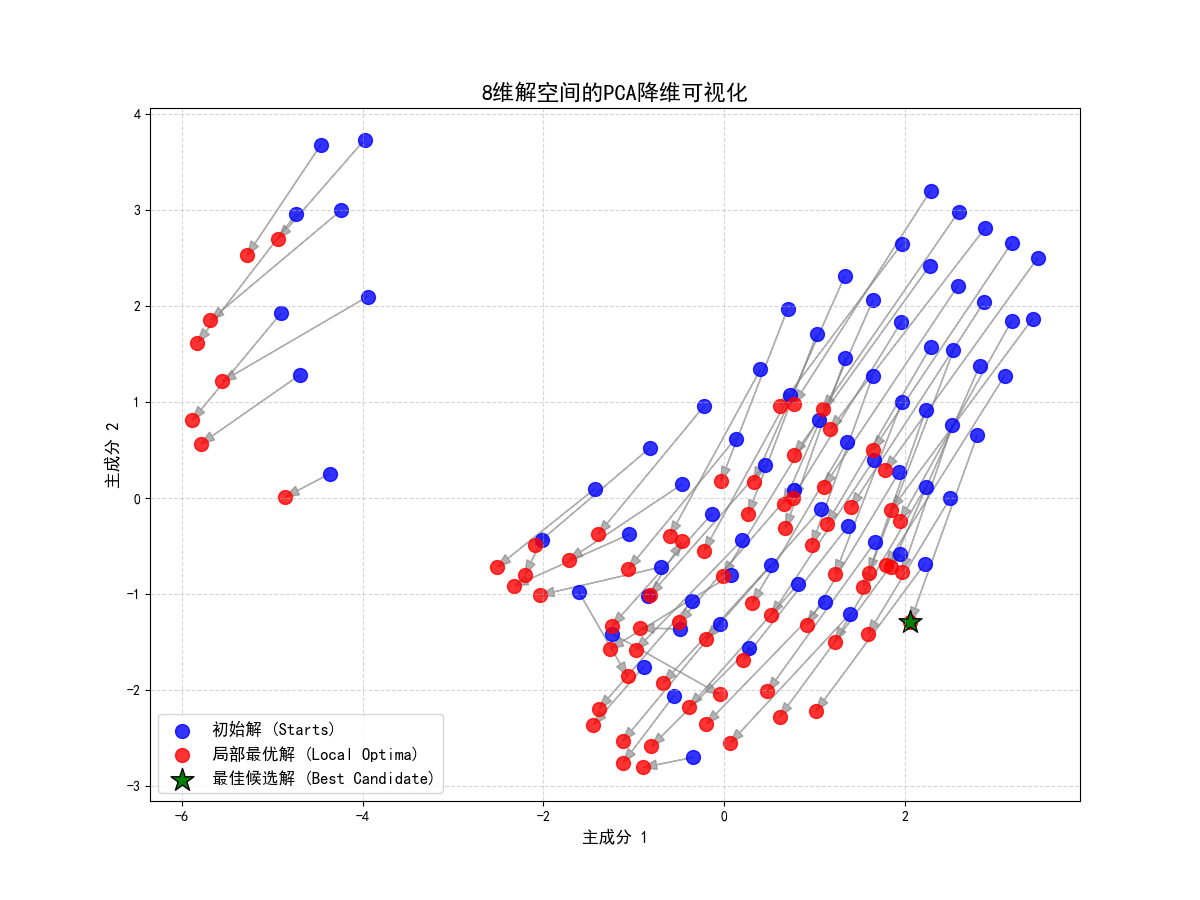
\includegraphics[width=\textwidth, height=0.25\textheight]{pic/Fg11.png}
					\caption{坐标上升法求解过程}
					\label{fig:pca_q3_right}
				\end{minipage}
			\end{figure}
			
			
			\item \textbf{最终测算与最优策略}: 对最佳候选解进行高精度测算后,得到问题三的最优干扰策略,详细参数与最终性能评估如表\ref{tab:results_q3}所示。
		\end{enumerate}
		
		% --- 插入您的Q3结果表格 ---
		\begin{table}[H]
			\centering
			\caption{问题三:最优干扰策略及最终结果}
			\label{tab:results_q3}
			\begin{tabular}{@{}llcc@{}}
				\toprule
				参数类别           & 变量                & 最优值      & 单位 \\ \midrule
				\textbf{UAV统一飞行策略} & 飞行速度 ($v$)        & 110.8789 & m/s  \\
				& 飞行方向 ($\theta$)     & 179.4645 & 度   \\ \midrule
				\textbf{第1枚烟幕弹} & 投放时间 ($t_{\text{drop1}}$) & 0.6146  & 秒   \\
				& 引信延迟 ($t_{\text{delay1}}$) & 3.6631  & 秒   \\ \midrule
				\textbf{第2枚烟幕弹} & 投放时间 ($t_{\text{drop2}}$) & 3.4152 & 秒   \\
				& 引信延迟 ($t_{\text{delay2}}$) & 4.6631  & 秒   \\ \midrule
				\textbf{第3枚烟幕弹} & 投放时间 ($t_{\text{drop3}}$) & 4.7752  & 秒   \\
				& 引信延迟 ($t_{\text{delay3}}$) & 5.0631  & 秒   \\ \midrule
				\textbf{最终性能评估} & \textbf{高精度总遮蔽时长} & \textbf{6.4460 } & \textbf{秒}   \\ \bottomrule
			\end{tabular}
		\end{table}
		
		通过程序模拟动画进一步验证,其演示结果如图\ref{fig:simulation_q3}所示。
		
		\begin{figure}[H]
			\centering
			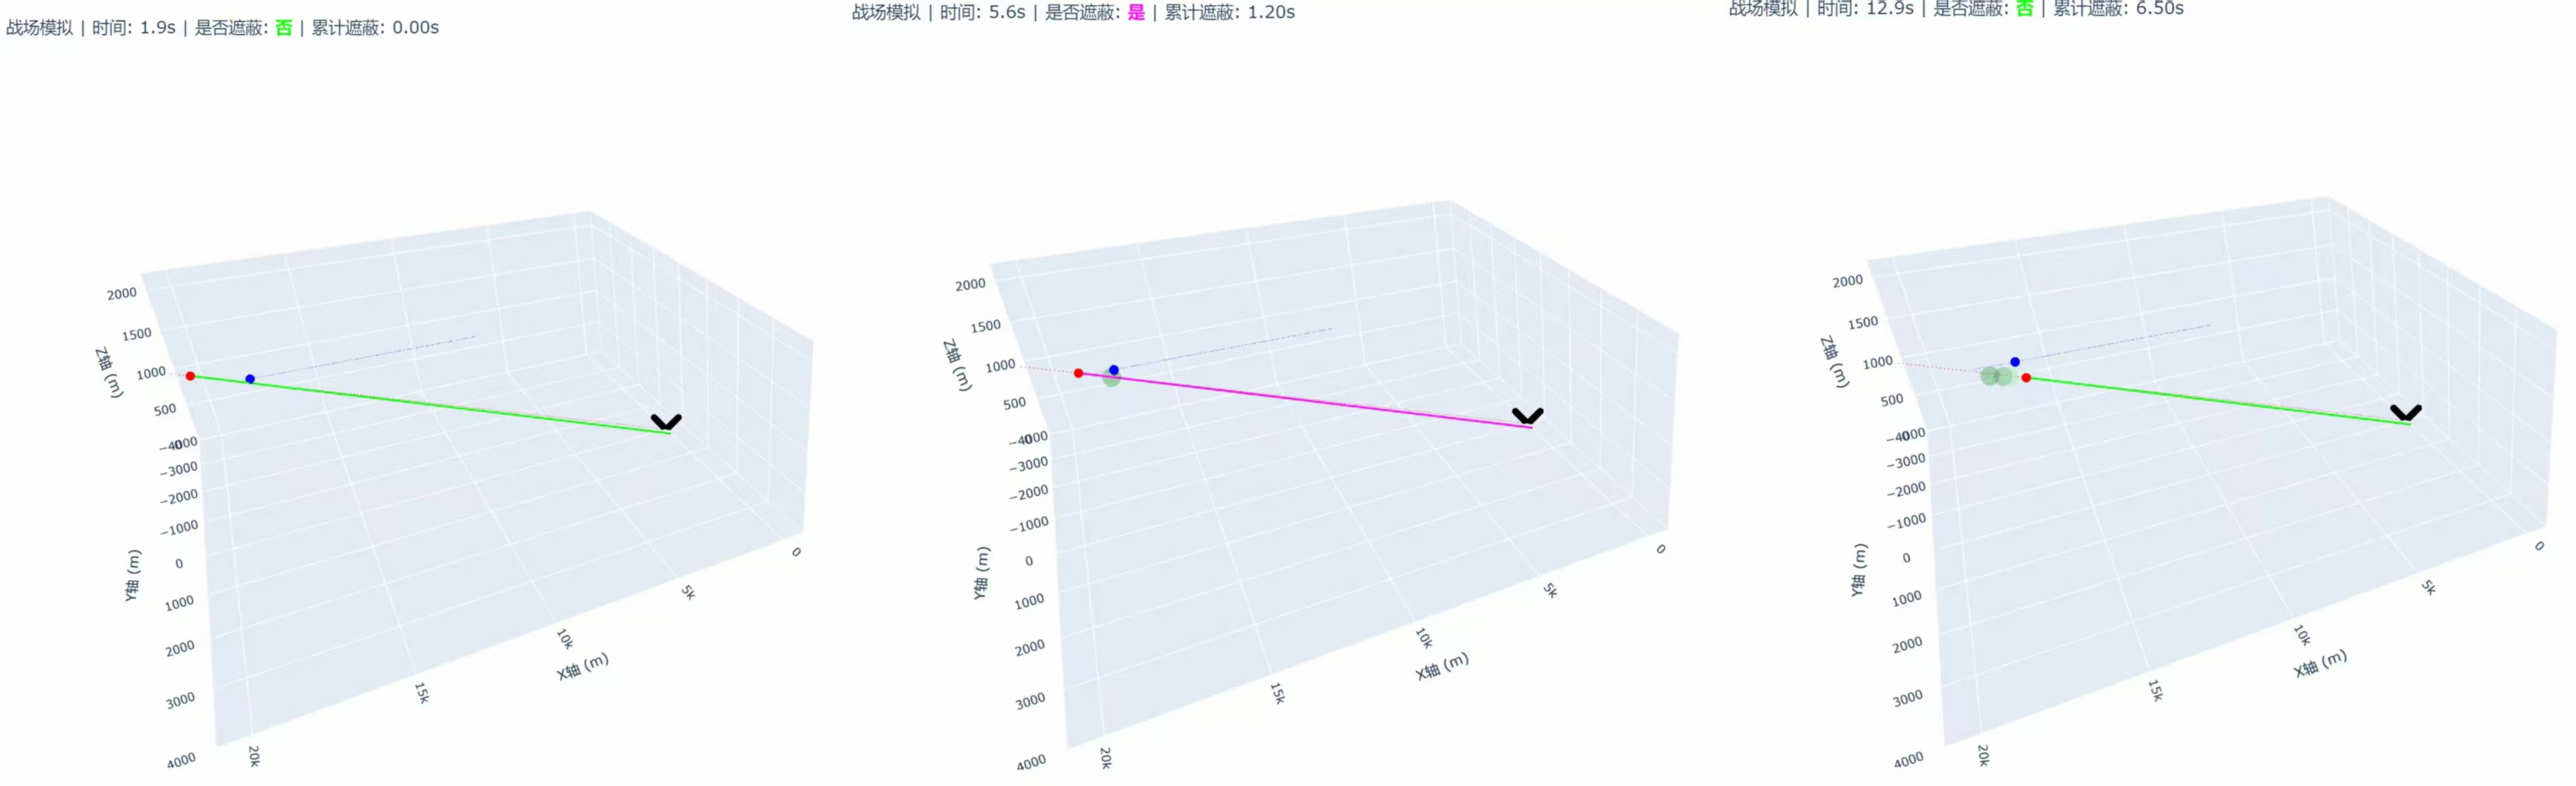
\includegraphics[width=0.9\textwidth]{pic/sim3.jpg}
			\caption{问题三程序模拟动画关键帧}
			\label{fig:simulation_q3}
		\end{figure}
		
		\subsection{问题四}
		
		
		问题四要求为三架初始位置不同的无人机协同规划干扰策略,是一个高维度的多智能体协同优化问题。决策变量的总维度达到了12维。高效求解这一问题,需要构建一个更为精妙和高效的\textbf{“多目标全局粗搜 $\rightarrow$ 贪心组合选择 $\rightarrow$ 协同局部精调 $\rightarrow$ 最终高精度测算”}四阶段分层优化框架。该框架的核心思想是“\textbf{分解-组合-协同}”。
		
		\subsubsection{四阶段分层优化框架}
		\paragraph{第一阶段:多目标全局粗搜}
		对三架无人机\textbf{分别独立}地执行问题二中的第一阶段全局粗搜,为每架无人机搜索并识别出50个最高质量的单兵作战策略,为后续组合提供高质量的参数组合。
		
		\paragraph{第二阶段:基于边际增益的贪心\cite{5}组合} 拥有了每个无人机的优秀策略后,理论组合数高达 $50^3$ 种。为高效筛选,设计一项\textbf{基于边际增益的贪心组合算法}。该算法优先考虑策略间的\textbf{互补性}。其核心逻辑是:
		
		\indent - \textbf{种子选择}: 以所有单机策略中最优的参数组合作为起点开启“团队组建”。\\
		\indent - \textbf{迭代增补}: 对于一个不完整的团队,遍历所有尚未加入的无人机及其策略,选择一个能够使当前团队\textbf{总协同遮蔽时长增益最大}的策略加入。边际增益的计算确保了每一步决策都是为了最大化团队的协同效应。\\
		\begin{equation}
			\text{MarginalGain}(S_{\text{new}}) = T_{\text{synergy}}(Team \cup \{S_{\text{new}}\}) - T_{\text{synergy}}(Team)
		\end{equation}
		\indent - \textbf{多起点组合与多样性维护}: 以多个不同的顶尖策略作为种子,生成50个不同的精英团队,并剔除相似组合,以保证进入下一阶段的初始解具有足够的多样性。
		
		
		\paragraph{第三阶段:高维局部精调}
		此阶段的目标是对每个精英团队的12个决策变量进行\textbf{联合微调}。我们采用\textbf{坐标上升法},但将其扩展至12维空间。在每一轮迭代中,算法会依次遍历全部12个决策变量,在其邻域内进行搜索,以找到使总协同遮蔽时长最大的新值。
		
		\paragraph{第四阶段:最终高精度测算。}
		与前几问一致,此阶段对最终方案进行最终计算。从第三阶段优化过的所有团队中,选取总协同遮蔽时长最长的组合作为答案,并采用包含1000个采样点的高精度目标模型计算其最终有效遮蔽时长。
		
		图\ref{fig:flowchart_q4}展示了问题四的完整的求解流程。
		
		\begin{figure}[H]
			\centering
			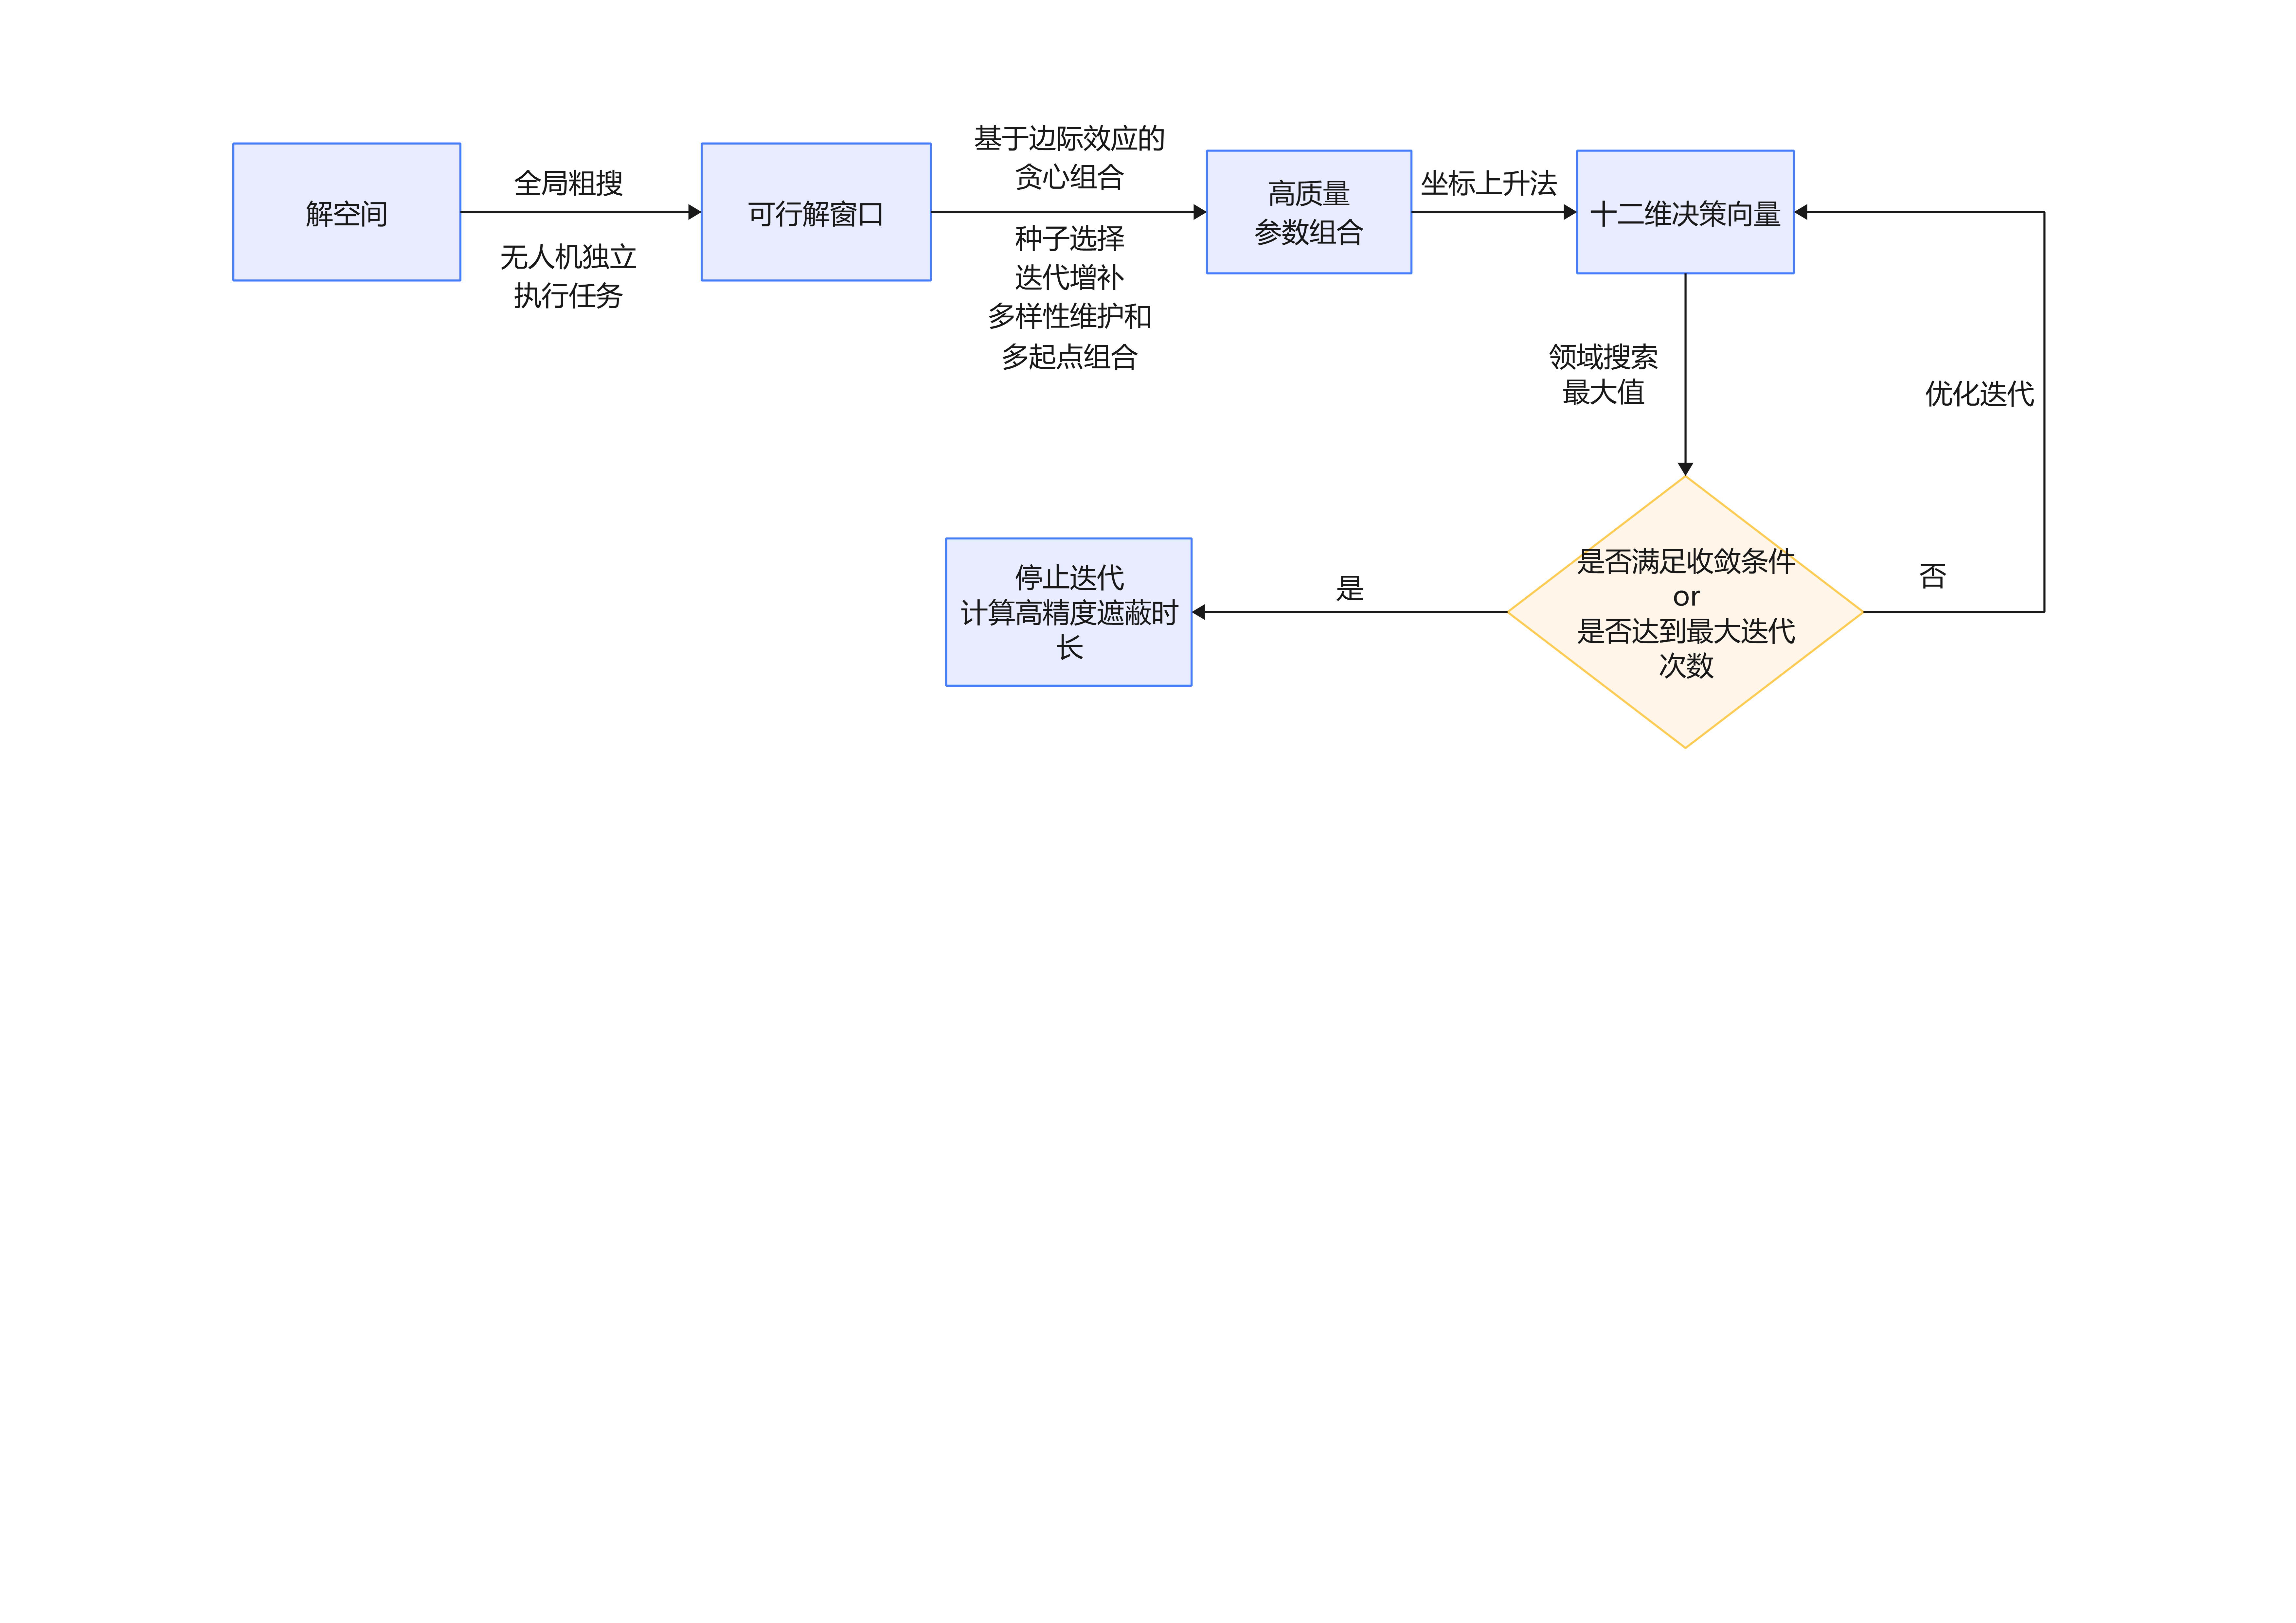
\includegraphics[width=0.8\textwidth]{pic/Fg8-Pb4.jpg}
			\caption{问题四求解流程图}
			\label{fig:flowchart_q4}
		\end{figure}
		
		
		\subsubsection{模型求解}
		程序严格按照四个阶段顺序执行,记录了贪心组合与局部精调阶段的关键中间数据,为算法的正确性和有效性提供了重要的过程依据。
		
		\begin{figure}[H]
			\centering
			\begin{minipage}[b]{0.48\textwidth}
				\centering
				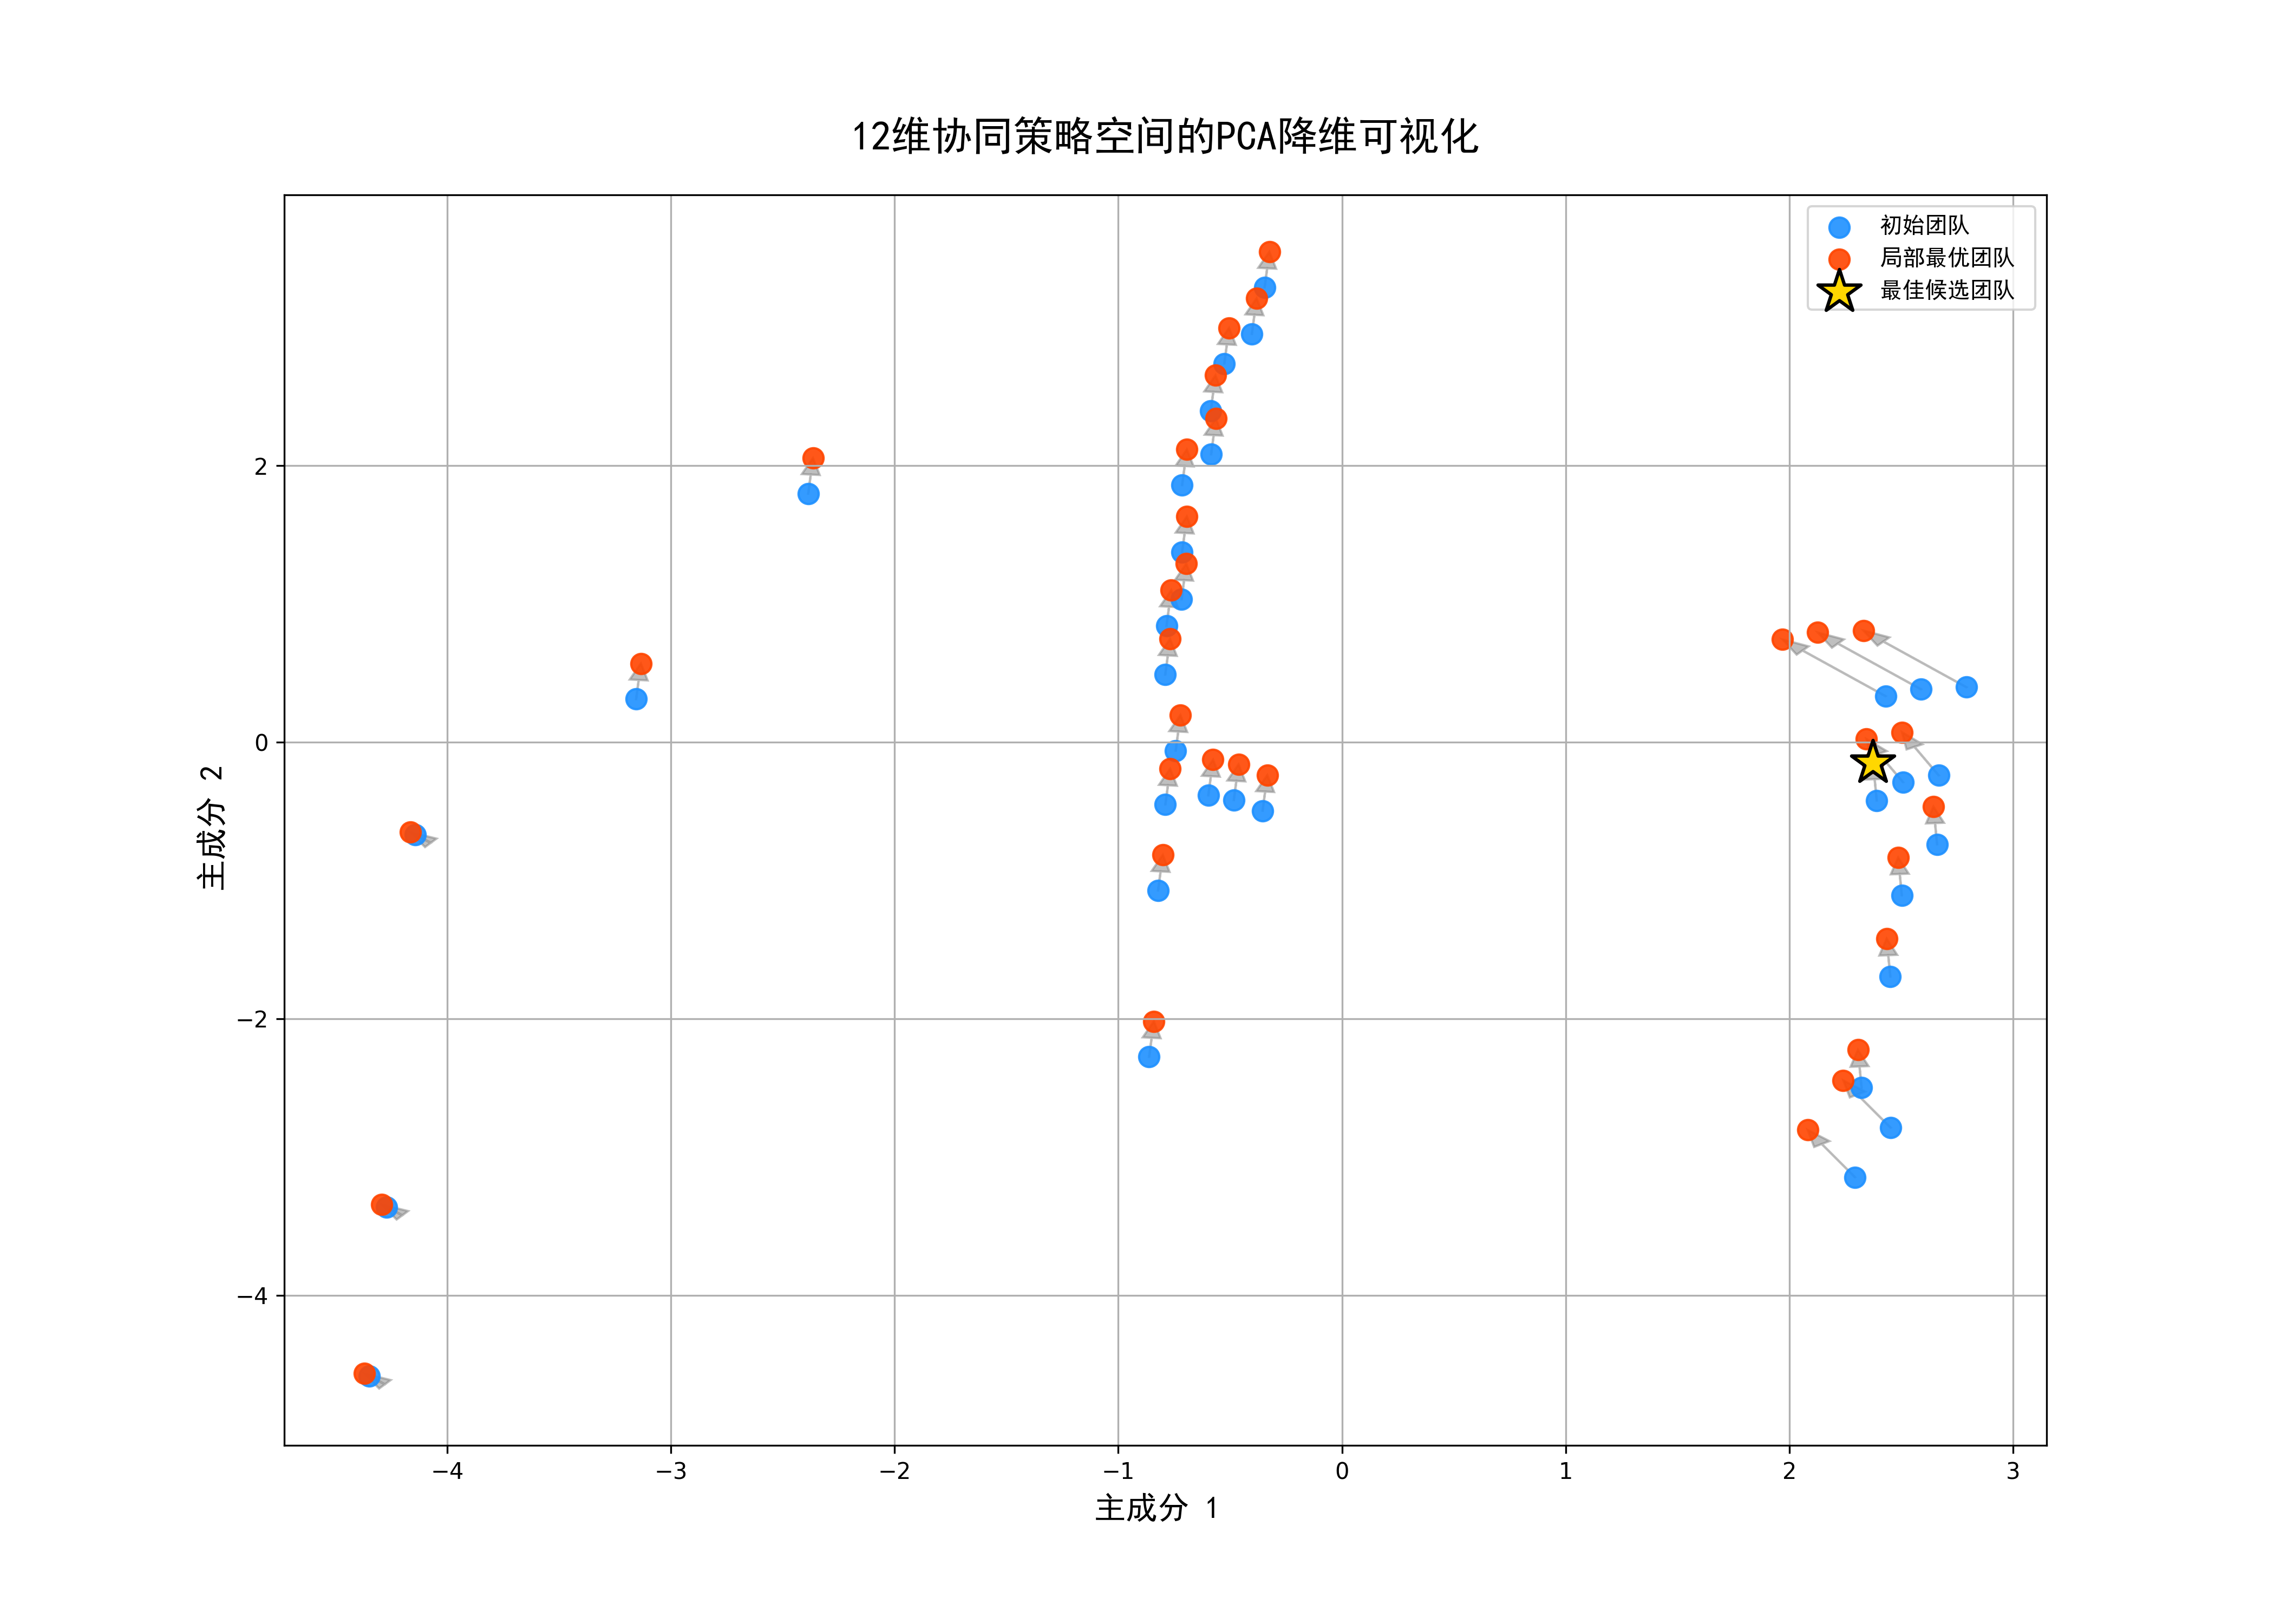
\includegraphics[width=\textwidth, height=0.25\textheight]{pic/Fg13.png}
				\caption{目标函数(遮蔽时长)的收敛情况}
				\label{fig:pca_q4_left}
			\end{minipage}
			\hfill
			\begin{minipage}[b]{0.48\textwidth}
				\centering					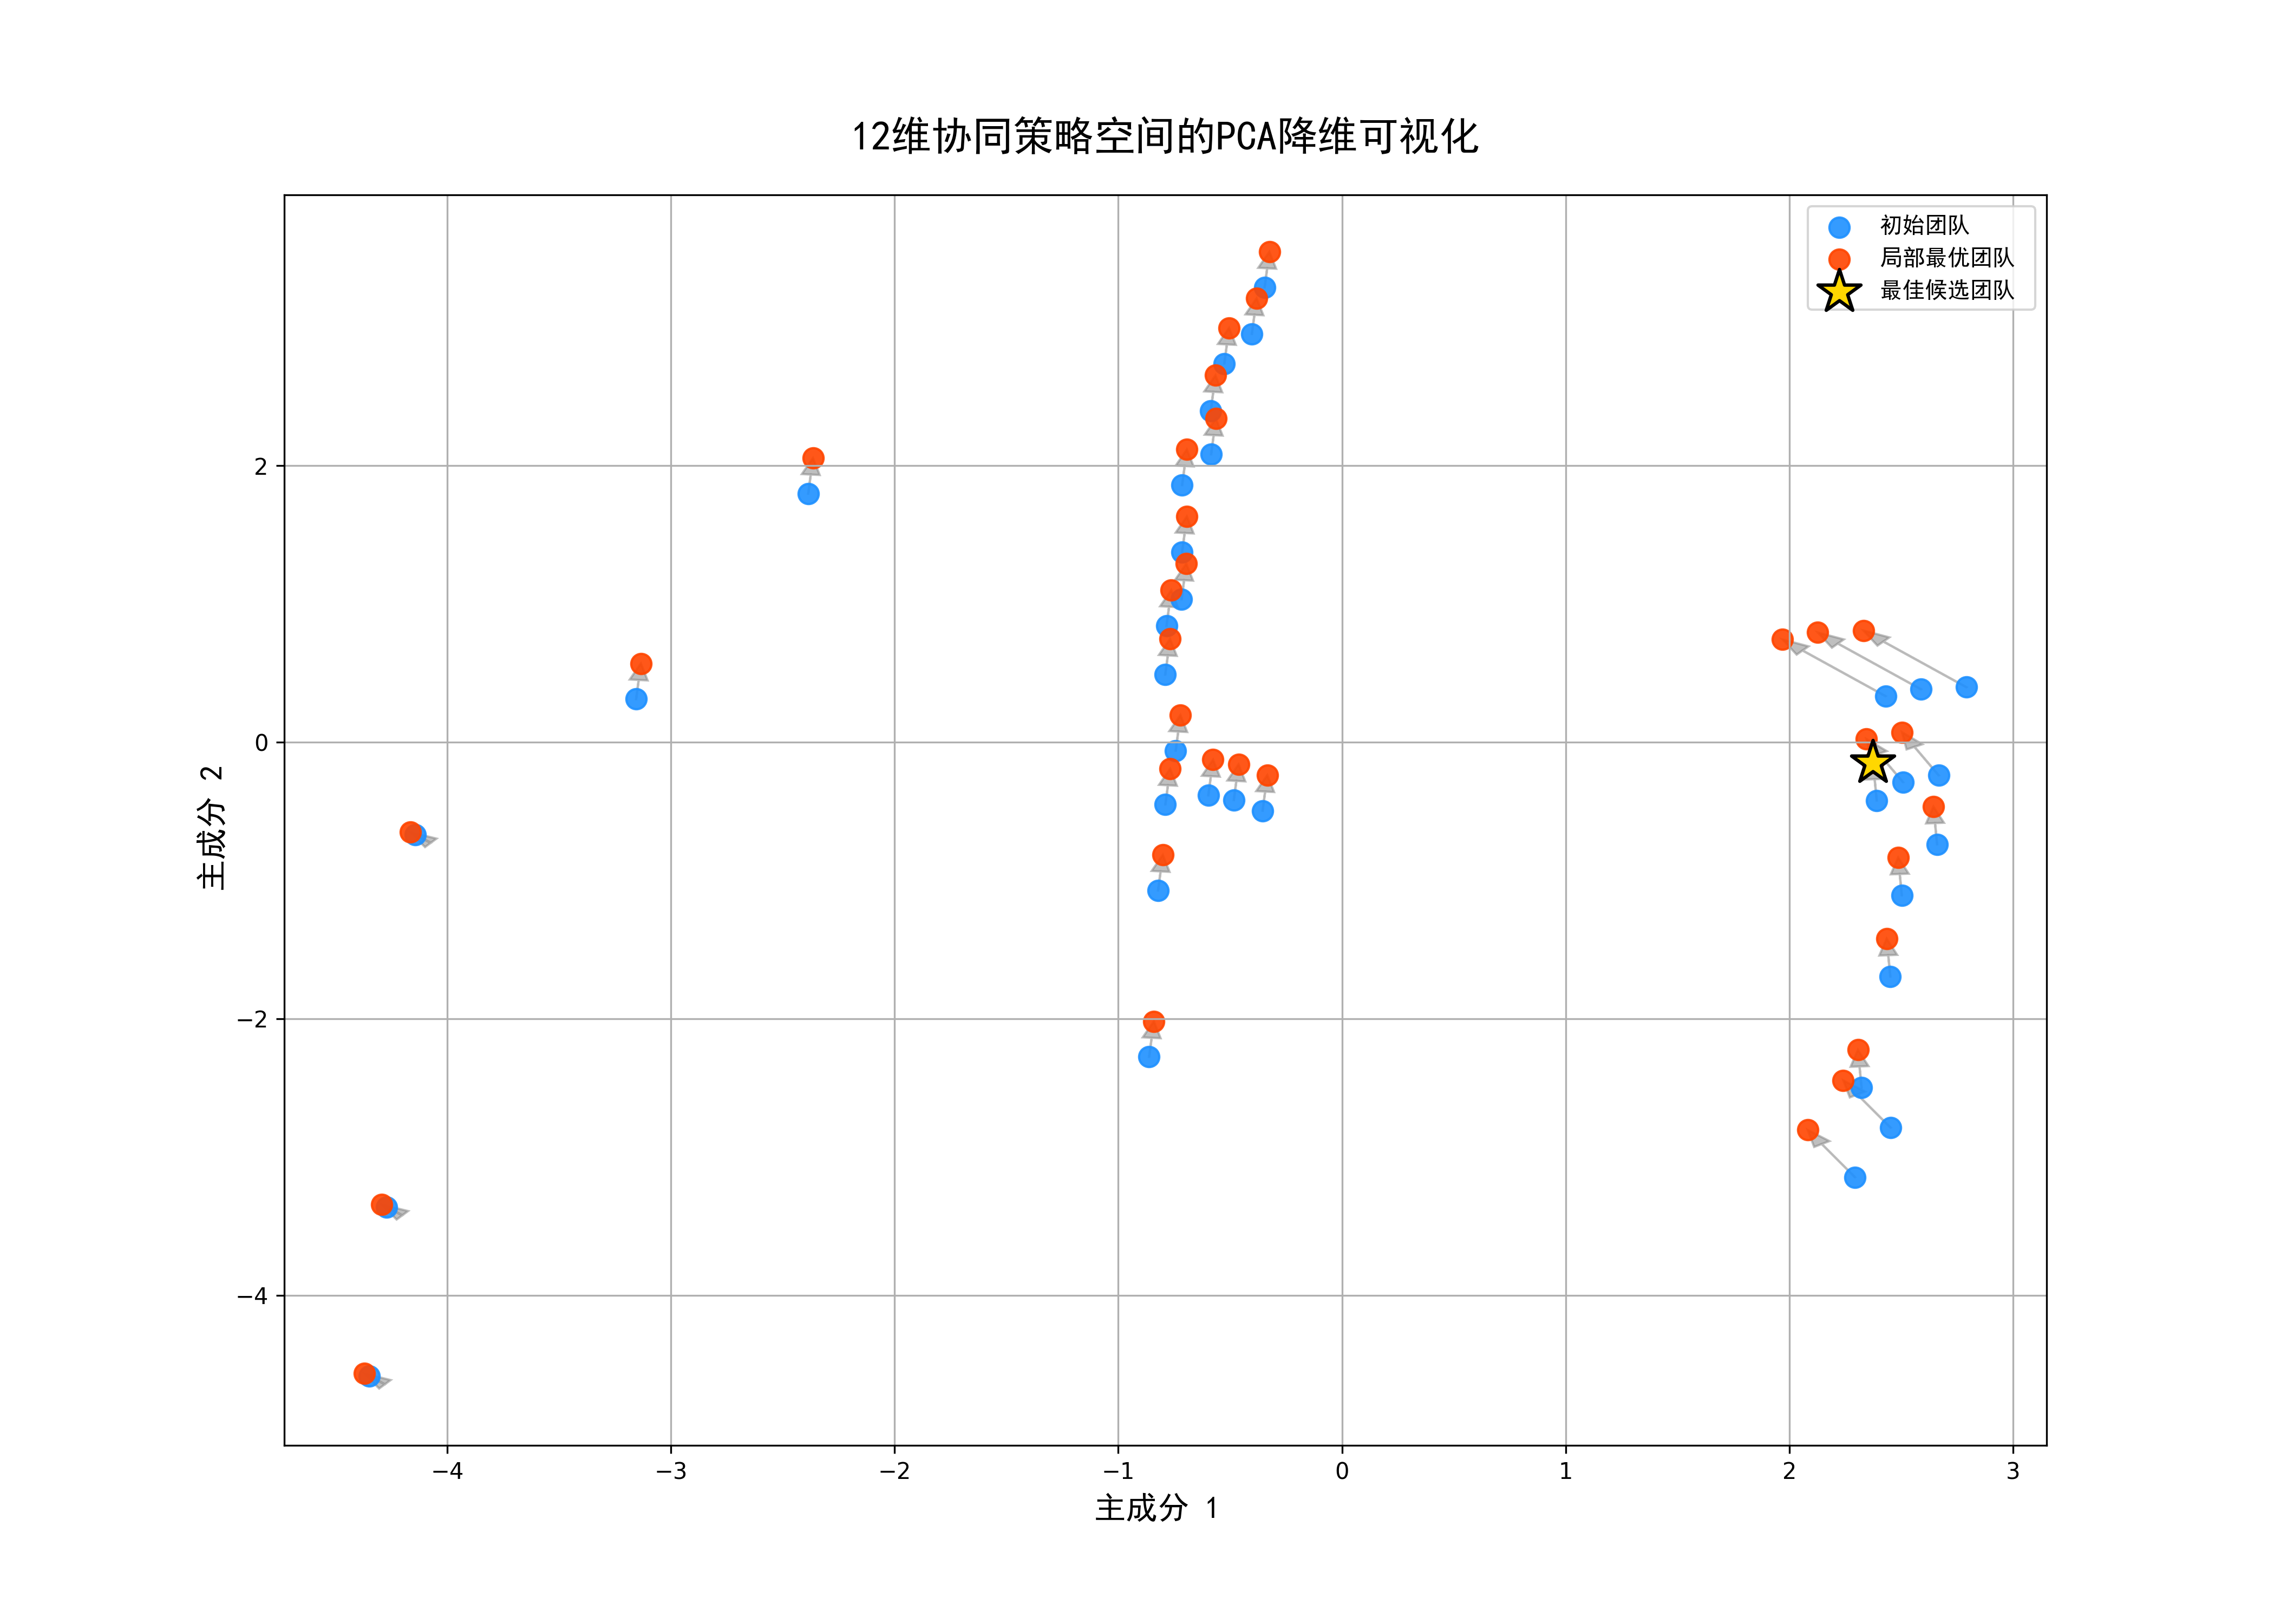
\includegraphics[width=\textwidth, height=0.25\textheight]{pic/Fg13.png}
				\caption{坐标上升法求解过程}
				\label{fig:pca_q4_right}
			\end{minipage}
		\end{figure}
		
		经过完整的四阶段求解流程,算法成功定位到最优协同干扰策略。对最终组合进行高精度测算后,得到的最优协同干扰策略详见表 \ref{tab:q4_results}。
		
		\begin{table}[H]
			\centering
			\caption{问题四:最优多机协同干扰策略}
			\label{tab:q4_results}
			%%\resizebox{\textwidth}{!}{%
				\begin{tabular}{@{}llcc@{}}
					\toprule
					\textbf{无人机} & \textbf{决策变量} & \textbf{最优值} & \textbf{单位} \\
					\midrule
					\textbf{FY1} & 飞行速度 ($v$) & 74.9189  & m/s \\
					& 飞行方向 ($\theta$) & 177.7362 & 度 \\
					& 投放时间 ($t_{\text{drop}}$) & 0.1334  & 秒 \\
					& 引信延迟 ($t_{\text{delay}}$) & 2.4883  & 秒 \\
					\midrule
					\textbf{FY2} & 飞行速度 ($v$) & 137.9929  & m/s \\
					& 飞行方向 ($\theta$) & 262.1467  & 度 \\
					& 投放时间 ($t_{\text{drop}}$) & 3.3801  & 秒 \\
					& 引信延迟 ($t_{\text{delay}}$) & 6.5017  & 秒 \\
					\midrule
					\textbf{FY3} & 飞行速度 ($v$) & 139.6679  & m/s \\
					& 飞行方向 ($\theta$) & 122.5601 & 度 \\
					& 投放时间 ($t_{\text{drop}}$) & 18.9682  & 秒 \\
					& 引信延迟 ($t_{\text{delay}}$) & 7.6522  & 秒 \\
					\midrule
					\textbf{最终性能评估} & \textbf{高精度总协同遮蔽时长} & \textbf{12.1670} & \textbf{秒} \\
					\bottomrule
			\end{tabular}
		\end{table}
		
		\begin{figure}[H]
			\centering
			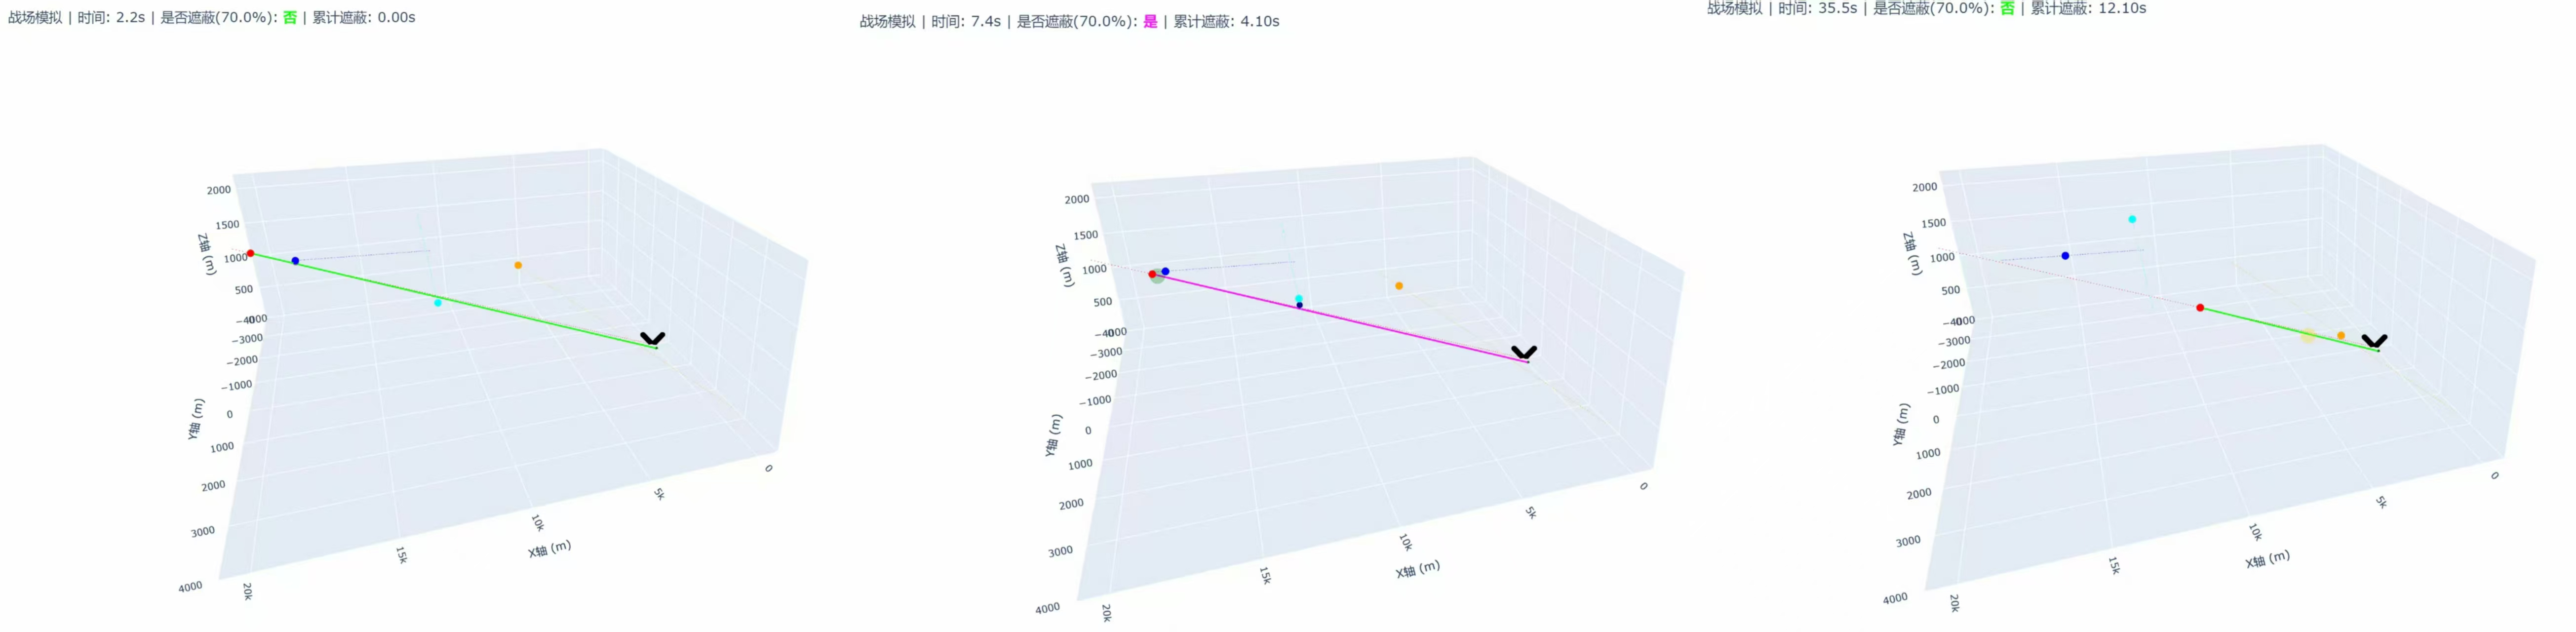
\includegraphics[width=0.8\textwidth]{pic/sim4.jpg}
			\caption{问题四程序模拟动画关键帧}
			\label{fig:simulation_q4}
		\end{figure}
		
		\subsection{问题五的模型建立与求解}
		问题五要求为五架无人机规划协同干扰策略,以应对三枚同时来袭的导弹。决策变量的总维度高达40维(5架无人机 × 8个决策变量),为高效求解此问题,我们在先前算法框架上改进设计了一个\textbf{“多目标全局粗搜 $\rightarrow$ 贪心组合选择 $\rightarrow$ 子问题降维与协同优化 $\rightarrow$ 最终高精度测算”}的四阶段分层优化框架。该框架首先将复杂的耦合问题分解为独立的子问题进行能力评估,然后通过智能的分配策略将问题降维,最后调用前几问已验证的成熟模型进行求解,最终实现全局最优目标。
		
		\subsubsection{四阶段分层优化框架}
		
		\paragraph{第一阶段:多目标全局粗搜}
		此阶段的目标是量化每一架无人机对每一枚来袭导弹的潜在干扰效能。我们遍历所有15种可能的“UAV-Missile”配对组合。对于每一种组合,我们求解单一无人机使用单枚烟幕弹对单一导弹进行干扰的最优遮蔽时长。这个过程通过调用一个类似于第二问的全局粗搜求解器来实现。最终,我们得到一个 $5 \times 3$ 的“效能矩阵” $E$,其中元素 $E_{ij}$ 代表第 $i$ 架无人机对第 $j$ 枚导弹的最大单弹干扰时长。
		
		\paragraph{第二阶段:基于边际增益的贪心任务分配}
		在获得效能矩阵后,我们需要为三枚导弹分配合计五架无人机,以实现总体效能最大化。我们借鉴问题四中基于边际增益的思想,设计了一套高效的贪心分配算法。其核心步骤如下:
		
		\begin{itemize}
			\item \textbf{主力分配:} 为确保每枚导弹都得到有效防御,算法首先从效能矩阵中找出数值最高的策略组合,为每枚导弹分配一个唯一的、对其最有效的无人机作为“主力防守者”。此步骤保证了基础防御覆盖。
			\item \textbf{辅助分配:} 分配完主力后,遍历每一架剩余的无人机,并评估它去干扰哪枚导弹能带来最大的“边际增益”。我们将无人机分配给能使其效能最大化的目标。
		\end{itemize}
		这一阶段完成后,我们就得到了一个明确的任务分配方案。
		
		\paragraph{第三阶段:子问题降维与协同优化}
		任务分配完成后,原先复杂的“五机三弹”问题被成功分解为三个独立的、规模更小的子问题:
		\begin{itemize}
			\item \textbf{单机多弹任务 (类似问题三):} 对于仅由一架无人机负责的导弹,问题转化为问题三的“单智能体、多次行为的协同优化”问题。我们直接应用问题三开发的三阶段优化模型,为该无人机规划最优的三弹投放策略。
			\item \textbf{双机多弹任务 (类似问题四的扩展):} 对于由两架无人机协同负责的导弹,问题转化为“多智能体、协同任务的策略优化”。这与问题四的场景类似,但扩展为每架无人机可投放三枚弹。我们为此场景构建了一个协同优化模型,对这两架无人机的全部16个决策变量进行联合局部精调,以最大化它们对目标导弹的协同遮蔽时长。
		\end{itemize}
		通过这种分配的方式,我们将一个难以直接求解的40维问题,分解为几个维度较低且已有成熟解决方案的子问题,大大提高了求解的效率和鲁棒性。
		
		\paragraph{第四阶段:最终高精度测算}
		在所有子问题都得到最优解后,我们将所有无人机的最优策略组合在一起,构成完整的最终方案。最后,我们运行一个全局高精度仿真,同时模拟三枚导弹和五架无人机的全部行动,得到最终的“总有效协同遮蔽时长”,作为对我们最终策略的性能评估。
		
		图\ref{fig:flowchart_q5}展示了问题五的完整的求解流程。
		
		\begin{figure}[H]
			\centering
			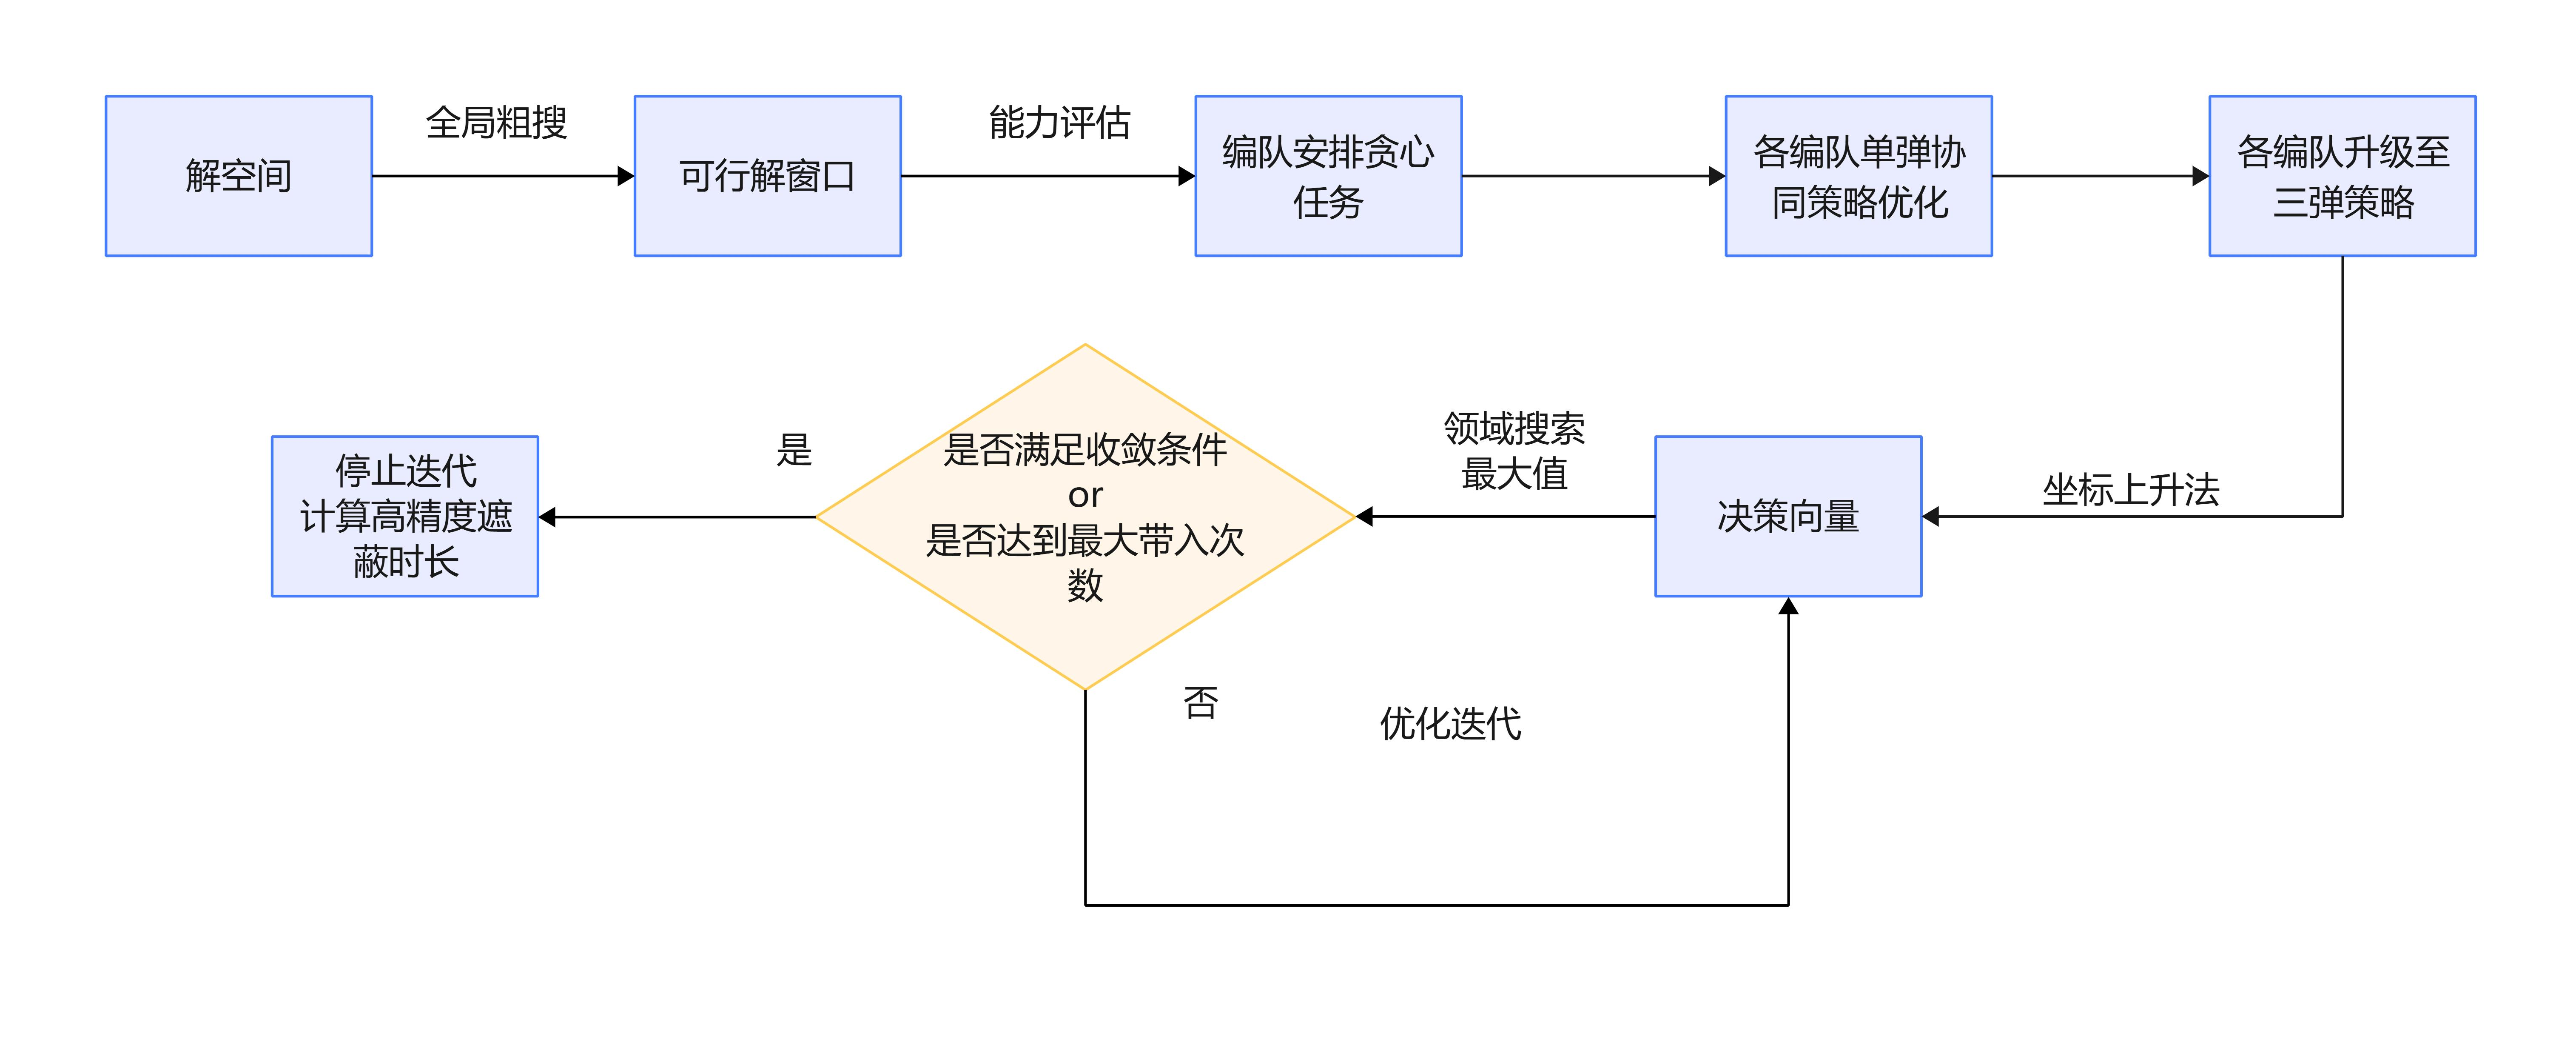
\includegraphics[width=0.8\textwidth]{pic/Pb5.jpg}
			\caption{问题五求解流程图}
			\label{fig:flowchart_q5}
		\end{figure}
		
		
		\subsubsection{模型求解与结果}
		我们严格按照上述四个阶段执行求解流程。
		\begin{enumerate}
			\item \textbf{能力评估与分配:} 首先并行计算得到 $5 \times 3$ 效能矩阵,并执行贪心分配算法。分配结果明确了每个无人机的作战目标。
			\item \textbf{降维求解:} 根据分配结果,对单机任务组和双机任务组分别调用对应的优化求解器,得到各小组的最优干扰策略。
			\item \textbf{结果汇总与测算:} 将所有策略汇总,并通过最终的高精度仿真模型进测算,得到最终结果。
		\end{enumerate}
		最优的五机三弹协同干扰策略及最终性能评估详见表5(这里我们列出了其中一组子问题的最优解,其余详见result3.xlsx)该策略充分利用了每架无人机的位置优势,并通过智能分配与协同优化,实现了对三枚来袭导弹的最大化干扰效果。
		
		\begin{table}[H]
			\centering
			\caption{问题五:最优多机协同干扰策略(针对导弹一)}
			\label{tab:q51_results}
			%%\resizebox{\textwidth}{!}{%
				\begin{tabular}{@{}llcc@{}}
					\toprule
					\textbf{无人机} & \textbf{决策变量} & \textbf{最优值} & \textbf{单位} \\
					\midrule
					\textbf{FY1} & 飞行速度 ($v$) & (填入您的结果) & m/s \\
					& 飞行方向 ($\theta$) & (填入您的结果) & 度 \\
					& 投放时间 ($t_{\text{drop}}$) & (填入您的结果) & 秒 \\
					& 引信延迟 ($t_{\text{delay}}$) & (填入您的结果) & 秒 \\
					\midrule
					\textbf{FY3} & 飞行速度 ($v$) & (填入您的结果) & m/s \\
					& 飞行方向 ($\theta$) & (填入您的结果) & 度 \\
					& 投放时间 ($t_{\text{drop}}$) & (填入您的结果) & 秒 \\
					& 引信延迟 ($t_{\text{delay}}$) & (填入您的结果) & 秒 \\
					\midrule
					\textbf{最终性能评估} & \textbf{高精度总协同遮蔽时长} & \textbf{(填入您的结果)} & \textbf{秒} \\
					\bottomrule
				\end{tabular}
			\end{table}
			
		\begin{figure}[H]
			\centering
			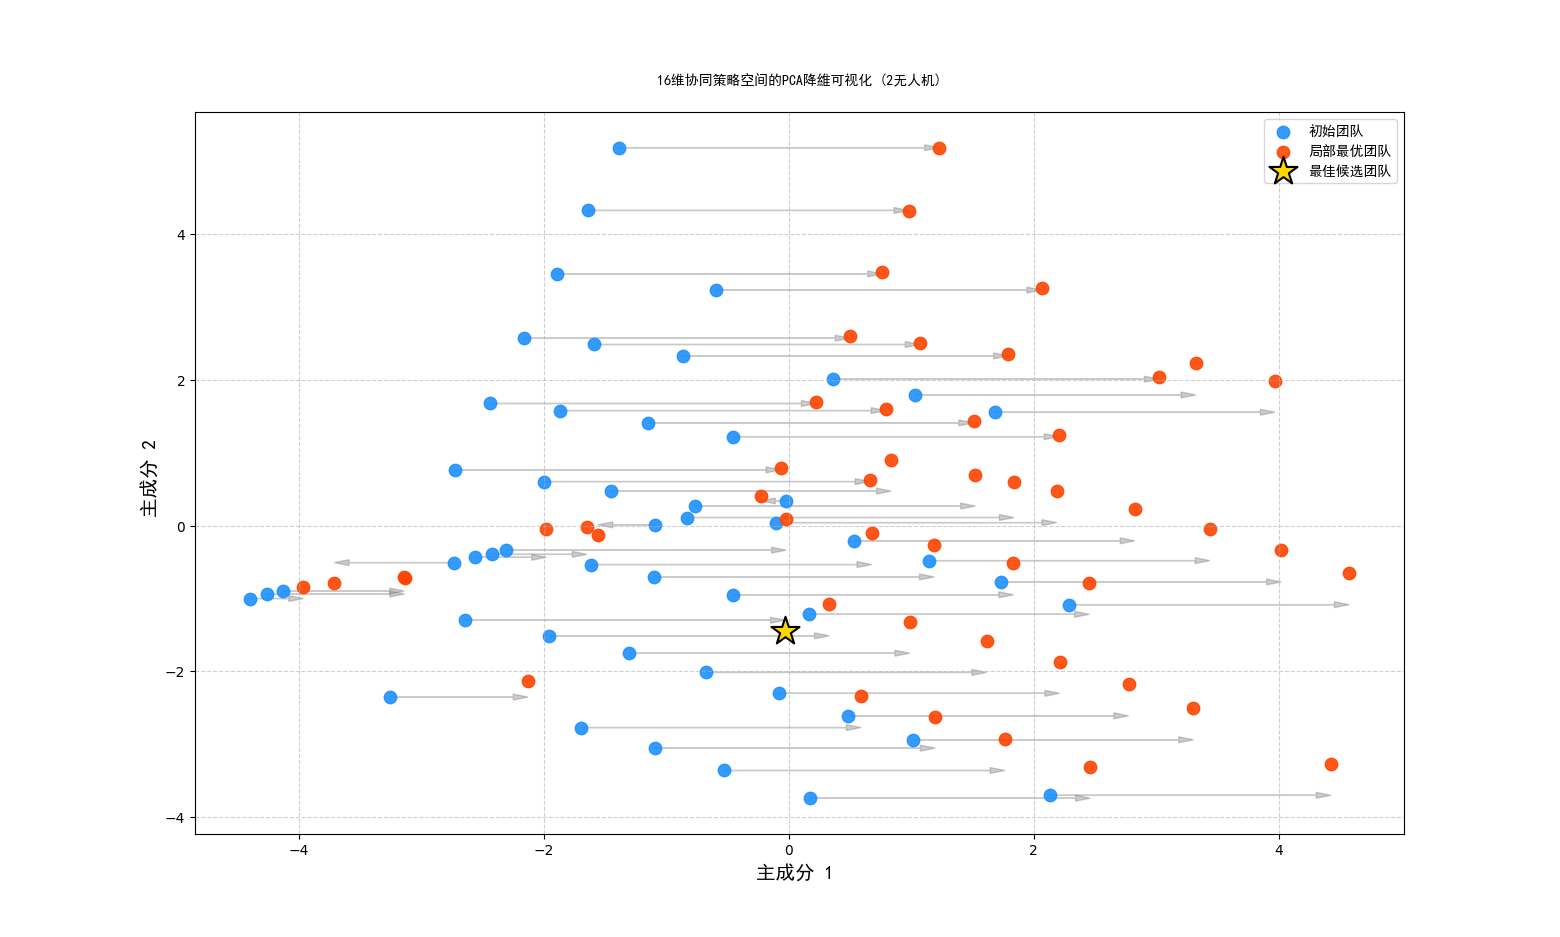
\includegraphics[width=0.8\textwidth]{pic/P51.png}
			\caption{问题五坐标上升法求解过程(FY1,FY2对M1)}
			\label{fig:pca5}
		\end{figure}
			
		\section{、模型的评价与推广}
		
		\subsection{模型的优点}
		\begin{enumerate}
			\item \textbf{框架设计创新且系统性强。} 本文针对问题复杂度递增的特点,设计了一套渐进式优化框架。该框架从问题二贯穿至问题五,成功地将高维、非凸的复杂优化问题分解为一系列可控的子步骤。
			
			\item \textbf{求解策略高效且鲁棒性高。} 针对解空间的非凸性,本文创新性地采用了“多起点”局部优化的策略。通过从多个高质量的初始解出发进行并行寻优,极大地降低了算法陷入低质量局部最优解的风险,保证了最终解的质量。
			
			\item \textbf{模型扩展性与可移植性强。} 本文建立的模型具有良好的模块化特性。我们能直接调用问题三与问题四的核心求解器去解决其他问题。这种“分而治之”和“降维打击”的思想,使得该模型框架具备推广潜力,可移植到其他类似的多智能体任务分配与协同路径规划问题中。
			
		\end{enumerate}
		
		\subsection{模型的不足}
		\begin{enumerate}
			\item \textbf{求解过程计算成本较高。} 本文在追求高质量解的过程中,全局搜索阶段和多起点优化策略需要遍历和迭代大量的参数组合。虽然提高了解的质量,但也耗费了大量的计算资源,延长了获得最终结果的时间。
			
			\item \textbf{启发式算法不保证全局最优。} 在问题四与问题五的任务分配环节,我们采用了基于边际增益的贪心算法。此类启发式算法的决策过程是链式的,每一步都选择当前最优,但这并不能从数学上保证最终的分配方案是全局最优解。
			
		\end{enumerate}
		
		\subsection{模型的推广}
		本研究提出的分层优化框架,特别是“分解-分配-降维-协同”的求解思想,具有广泛的应用价值。该框架可推广至:
		\begin{itemize}
			\item \textbf{其他无人机集群任务:} 如多无人机协同侦察、多目标打击、物流配送网络优化等,只需替换底层的物理模型和目标函数即可。
			\item \textbf{资源调度与分配问题:} 如通信网络中的信道分配、计算中心的任务调度等,其中“能力评估-贪心分配”的逻辑可以被直接借鉴。
			\item \textbf{机器人协同作业:} 在自动化仓储、智能工厂等场景下,多机器人需要协同完成复杂任务,本模型的框架可为其路径规划和任务分配提供有效的解决方案。
		\end{itemize}
		
		
		
		\newpage
		
		
		\begin{thebibliography}{99}
			

			\bibitem{1} 罗瑞耀,王得霖,罗威,等. 烟幕弹应对察打一体无人机的投放策略研究[J].光电技术应用,2022,37(06):90-98.
			
			\bibitem{2} 代敏.烟幕干扰下的地面目标识别算法研究[D].华中科技大学,2020.DOI:10.27157/d.cnki.ghzku.2020.002800.
			
			\bibitem{3}花超,廖守亿,张作宇,等. 烟幕对红外导引头干扰效果仿真研究[J].激光与红外,2019,49(02):217-221.

			\bibitem{4}顾文慧,高红杰. 烟幕投放控制分析与设计[J].光电技术应用,2014,29(02):87-89.
			
			\bibitem{5}常友渠,肖贵元,曾敏. 贪心算法的探讨与研究[J].重庆电力高等专科学校学报,2008,(03):40-42+47.
			
		\end{thebibliography}
		
		\clearpage
		
		\setcounter{page}{1} % 附录页码从1开始
		
		
		\section*{附录}
		
		\subsection*{1.支撑材料列表}
		
		\begin{figure}[H]
		%%	\centering
			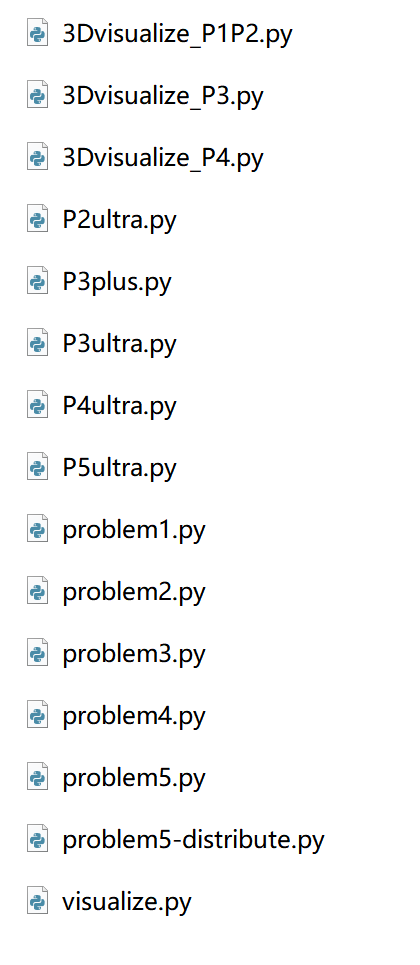
\includegraphics[width=0.4\textwidth]{pic/zhicheng.png}
		\end{figure}		
		
		\begin{figure}[H]
			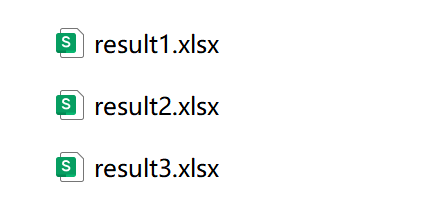
\includegraphics[width=0.4\linewidth]{pic/zc2}
		\end{figure}
		
		\newpage
		\subsection*{2.主要程序代码(部分)}
		
		
	\end{CJK}
\end{document}
